\documentclass[10pt,oneside]{article}
\usepackage[margin=0.82in]{geometry}
\usepackage{fontspec}
\setmainfont{DejaVu Serif}
\setsansfont{DejaVu Sans}
\setmonofont{DejaVu Sans Mono}[Scale=0.88]
\usepackage{amsmath,amssymb,amsthm,mathtools}
\usepackage{booktabs,longtable,array,multirow,tabularx}
\usepackage{enumitem}
\usepackage[table]{xcolor}
\usepackage{hyperref}
\usepackage{cleveref}
\usepackage{listings}
\usepackage{fancyhdr}
\usepackage{titlesec}
\usepackage{microtype}
\usepackage{tikz}
\usetikzlibrary{arrows.meta,positioning,fit,calc,shapes.geometric}
\usepackage{caption}
\usepackage{graphicx}
\usepackage{setspace}
\usepackage[most]{tcolorbox}
\usepackage{etoolbox}
\setcounter{secnumdepth}{0}
\setcounter{tocdepth}{2}
\setlength{\headheight}{14pt}
\hypersetup{colorlinks=true,linkcolor=blue!45!black,citecolor=blue!45!black,urlcolor=blue!45!black,pdfauthor={Ian Farquharson},pdftitle={Synthetic Cognitive Coding (SCC): Formal Constitutional-Operational Specification - Final Canon - Scholarly Edition}}
\pagestyle{fancy}
\fancyhf{}
\lhead{Synthetic Cognitive Coding (SCC)}
\rhead{Formal Constitutional-Operational Specification}
\cfoot{\thepage}
\setlist[itemize]{topsep=3pt,itemsep=2pt,parsep=1pt,leftmargin=1.45em}
\setlist[enumerate]{topsep=3pt,itemsep=2pt,parsep=1pt,leftmargin=1.65em}
\lstset{basicstyle=\ttfamily\footnotesize,breaklines=true,columns=fullflexible,keepspaces=true,frame=single,framerule=0.25pt,xleftmargin=0.5em,xrightmargin=0.5em}
\titleformat{\section}{\Large\bfseries}{\thesection}{0.75em}{}
\titleformat{\subsection}{\large\bfseries}{\thesubsection}{0.75em}{}
\titleformat{\subsubsection}{\normalsize\bfseries}{\thesubsubsection}{0.75em}{}
\newtheorem*{theorem}{Theorem}
\newtheorem*{proposition}{Proposition}
\newtheorem*{corollary}{Corollary}
\newtheorem*{lemma}{Lemma}
\theoremstyle{definition}
\newtheorem*{definition}{Definition}
\newtheorem*{assumption}{Assumption}
\theoremstyle{remark}
\newtheorem*{remark}{Remark}
\newcommand{\N}{\mathbb{N}}
\newcommand{\B}{\mathbb{B}}
\newcommand{\R}{\mathbb{R}}
\newcommand{\one}{\mathbf{1}}
\newcommand{\Lip}{\operatorname{Lip}}
\newcommand{\Sh}{\mathrm{Sh}}
\newcommand{\PO}{\mathrm{PO}}
\newcommand{\Abs}{\mathrm{Abs}}
\newcommand{\Impl}{\mathrm{Impl}}
\newcommand{\safe}{\mathrm{safe}}
\newcommand{\prot}{\mathrm{prot}}
\newcommand{\mem}{\mathrm{mem}}
\newcommand{\hash}{\mathrm{hash}}
\newcommand{\mode}{\mathrm{mode}}
\newcommand{\task}{\mathrm{task}}
\newcommand{\cmp}{\mathrm{cmp}}
\newcommand{\AUD}{\mathrm{AUD}}
\newcommand{\RISK}{\mathrm{RISK}}
\newcommand{\Next}{\mathrm{Next}}
\newcommand{\dom}{\mathrm{dom}}
\newcommand{\id}{\mathrm{id}}
\newcommand{\inv}{\mathrm{inv}}
\newcommand{\gov}{\mathrm{gov}}
\newcommand{\risk}{\mathrm{risk}}
\newcommand{\audit}{\mathrm{audit}}
\newcommand{\iso}{\mathrm{iso}}
\newcommand{\refine}{\mathrm{refine}}
\newcommand{\Exact}{\mathrm{Exact}}
\newcommand{\Stutter}{\mathrm{Stutter}}
\newcommand{\SafeRefined}{\mathrm{SafeRefined}}
\newcommand{\bt}{\begin{theorem}}
\newcommand{\et}{\end{theorem}}
\newcommand{\ThScope}[3]{\par\smallskip\noindent{\normalfont\small\textbf{Scope and dependencies.} \textit{Scope:} #1 \textit{Dependencies:} #2 \textit{Status:} #3}\par\smallskip}
\newcommand{\reviewtarget}[1]{\texttt{\detokenize{#1}}}
\newcommand{\leantarget}[2]{\begin{tabular}[t]{@{}l@{}}\footnotesize\texttt{\detokenize{#1}}\\[-1pt]\footnotesize\texttt{\detokenize{#2}}\end{tabular}}
\newcommand{\mechtarget}[3]{\begin{tabular}[t]{@{}l@{}}\scriptsize\texttt{\detokenize{#1}}\\[-1pt]\scriptsize\texttt{\detokenize{#2}}\\[-1pt]\scriptsize\emph{#3}\end{tabular}}
\newcolumntype{Y}{>{\raggedright\arraybackslash}X}
\newcolumntype{Z}[1]{>{\raggedright\arraybackslash}p{#1}}

\linespread{1.015}
\definecolor{sccBlue}{RGB}{24,56,89}
\definecolor{sccGold}{RGB}{128,96,32}
\definecolor{sccRed}{RGB}{120,32,32}
\definecolor{sccSoftBlue}{RGB}{240,246,252}
\definecolor{sccSoftGold}{RGB}{252,248,236}
\newtcolorbox{hallofshame}{breakable,colback=red!3,colframe=sccRed!70!black,title={Hall of Shame: Misreadings That Kill Systems},fonttitle=\bfseries,boxrule=0.55pt,arc=1.5mm,left=1.2mm,right=1.2mm,top=1mm,bottom=1mm}
\newtcolorbox{kernelbox}{breakable,colback=sccSoftBlue,colframe=sccBlue!75!black,boxrule=0.45pt,arc=1.5mm,left=1.5mm,right=1.5mm,top=1mm,bottom=1mm}
\newcommand{\PartIntro}[1]{\noindent\textbf{In this part.} #1\par\medskip}
\newcommand{\WhyMatters}[1]{\par\smallskip\noindent\textbf{Why this matters.} #1\par}
\newcommand{\Intuition}[1]{\par\smallskip\noindent\textbf{Intuition.} #1\par\smallskip}
\newcommand{\RiskCritical}{\cellcolor{red!18}\textbf{Critical}}
\newcommand{\RiskHigh}{\cellcolor{orange!18}\textbf{High}}
\newcommand{\RiskMedium}{\cellcolor{yellow!22}\textbf{Medium}}
\AtBeginEnvironment{theorem}{\setstretch{1.03}}
\AtBeginEnvironment{proposition}{\setstretch{1.03}}
\AtBeginEnvironment{corollary}{\setstretch{1.03}}
\AtBeginEnvironment{proof}{\setstretch{1.03}}


\begin{document}
\begin{titlepage}
\centering
{\Huge\bfseries Synthetic Cognitive Coding (SCC)\\[0.35em]}
{\LARGE Formal Constitutional-Operational Specification\\[0.25em]}
{\Large Final Canon --- Scholarly Edition\\[1.15em]}
{\large Written by Ian Farquharson}\\[0.25em]
{\normalsize Emergent-Evo Engineer \textbar{} Neural-Synth Architect}\\[1.25em]
{\normalsize Logo asset preserved by reference: \url{https://gist.github.com/user-attachments/assets/0b9fbc2b-ae9c-4a68-989c-84bae78849dc}}\\[2em]
\vfill
{\large Canonical manuscript date: April 26, 2026}\\[1em]
{\normalsize Copyright \copyright{} 2025--2026 Ian Farquharson}\\[0.5em]
{\normalsize Licensed under the Creative Commons Attribution-ShareAlike 4.0 International License (CC BY-SA 4.0).}\par
{\normalsize License URL: \url{https://creativecommons.org/licenses/by-sa/4.0/}}\\[1em]
{\small Official author-published versions constitute the authoritative SCC canon. Pre-canonical gists, implementation guides, and associated developmental materials remain historical and archival artifacts unless expressly designated by the author as canonical.}
\end{titlepage}

\pagenumbering{roman}
\section*{Abstract}
Synthetic Cognitive Coding (SCC) is a typed, multi-sorted constitutional-operational calculus for governing sovereign, self-modifying cognitive systems. The specification organizes constitutional clauses, operational transition laws, proof-obligation bundles, refinement mappings, audit determinism, memory and lineage laws, risk escalation, halt absorption, and distributed quorum conditions into a single formal kernel. A lawful ordinary step is defined by well-typedness, domain admissibility, hard-clause preservation, structural non-interference, audit legibility, lineage continuity, and production of checkable witnesses. SCC separates three categories that must remain logically distinct: mathematical theorems proved under explicit hypotheses, constitutional declarations that bind as governing law, and external implementation assumptions such as cryptographic integrity, network synchrony, structural-isolation semantics, and verifier correctness. The mathematical core includes a weighted product metric on the non-protected state space, a lifted pseudometric on the full state space, well-posed deterministic trajectory semantics, a seven-stage execution pipeline, Lipschitz composition bounds, uniform contraction and incremental stability results, weighted small-gain criteria, governance projection laws, halt absorption, deterministic compression entropy monotonicity for discrete Shannon entropy, replay determinism, monotone refinement preservation, pointwise trace compliance, and conditional quorum safety for federated deployments. The result is a claim-scoped specification intended for formal review, proof-assistant mechanization, implementation audit, and independent verification.

\section{Introduction}
Self-modifying cognitive systems create a governance problem ordinary software safety arguments cannot touch. A system that can rewrite its own policies, memory structures, tool interfaces, execution paths, or federation rules can silently drift from its original identity while still producing plausible outputs.

Three failure modes dominate: 
\emph{sovereign drift}---the system becomes governed by a different constitution without announcement; 
\emph{audit collapse}---the history required to reconstruct lawfulness is lost, compressed beyond recovery, or rendered non-canonical; 
and \emph{governance capture}---ordinary optimization, updates, or federation logic quietly erode the hard constraints meant to bind it.

Existing approaches fall short. Prompt policies and output filters constrain surface behavior but define no typed transition law. Preference learning and constitutional training shape outputs but supply no replayable proof obligation per step. Classical formal methods verify kernels or protocols but rarely separate constitutional law, mathematical theorems, and external assumptions inside one governance calculus. Distributed quorum protocols prevent conflicting certificates under their assumptions but do not define what makes a cognitive state transition lawful.

SCC does not claim a metric or constitution magically solves deployment. It defines the exact conditions under which an ordinary step is lawful---typed, domain-admissible, hard-clause preserving, structurally non-interfering, audit-legible, lineage-preserving, and backed by a checkable proof-obligation bundle---and rejects everything else with prejudice.

The specification then binds that step discipline to contraction and small-gain analysis, governance projection, halt absorption, replay determinism, refinement, pointwise compliance, and conditional federation safety.

Read SCC as a constitutional-operational kernel, not a training method, alignment slogan, or blanket safety claim. Theorems hold only under their stated hypotheses. Constitutional clauses bind as governing law. Cryptographic integrity, verifier correctness, structural-isolation semantics, and network assumptions remain external until separately verified. This three-order separation is the primary defense against category error: SCC proves what can be proved, declares what binds as law, and explicitly names what remains assumed — with zero tolerance for conflation.

\subsection*{Keywords}
Synthetic Cognitive Coding; formal methods; constitutional AI governance; self-modifying systems; proof obligations; refinement; audit determinism; lineage; contraction mappings; small-gain theorem; Byzantine quorum safety; Lean 4 mechanization.

\subsection*{Paper Classification}
This manuscript is best classified as a formal-methods specification and constitutional-operational systems paper. It combines axiomatic governance clauses, typed transition semantics, dynamical-systems stability arguments, refinement and simulation theory, audit/replay laws, and conditional distributed-systems safety theorems.

\subsection*{Status of This Canonical Edition}
This is the author-designated scholarly canon for SCC. It controls terminology, state spaces, transition laws, invariants, proof obligations, refinement, compliance theorems, mechanization targets, and assumption boundaries. Each substantive claim carries a status: theorem, constitutional clause, meta-formal rule, implementation assertion, or external assumption.

\subsection*{How to Read This Document}
Readers new to SCC should begin with the Executive Summary, Document Scope and Use, Academic Contributions, and Design Rationale before moving to the formal articles. Parts I--III establish the typing discipline and constitutional commitments. Parts IV--VIII state the state-space, metric, transition, stability, memory, replay, refinement, and compliance core. Parts IX--XIII address federation, mechanization, assumptions, implementation validation, and machine-checking boundaries. The appendices provide a compact reference, provenance record, review checklist, glossary, final statement of intent, license notice, and bibliographic context.

\subsection*{Acknowledgments}
This edition acknowledges Dr. Robert Whetsel for early mentorship and Vlad Puscoiu for terminal basics.\
{\footnotesize Reference links: \url{https://www.linkedin.com/in/robertwhetsel}; \url{https://nl.linkedin.com/in/vlad-puscoiu-152436246}.}

\tableofcontents
\listoffigures
\listoftables
\newpage
\pagenumbering{arabic}


\section{Executive Summary}
Synthetic Cognitive Coding (SCC) is a constitutional runtime kernel for self-modifying systems.

An adaptive cognitive system is not governed because it sounds safe. Governance exists only when every ordinary step is typed, witnessed, checked, replayable, and rejected the instant the proof-obligation bundle fails.

SCC is not a prompt policy, preference patch, output filter, or after-the-fact audit story. It defines a formal kernel for sovereign, self-modifying cognitive systems: individual agents, tool-using runtimes, memory-bearing assistants, and federations of interacting nodes. The kernel binds state, law, proof obligation, audit, lineage, risk, halt, refinement, and distributed coherence into one claim-scoped specification.

The proof-obligation bundle and its fail-closed checker form SCC's enforcement core. No bundle, no acceptance. No acceptance, no output, no state promotion, no audit commit. A rejected bundle is not a warning; it terminates ordinary lawfulness for that candidate step. See Articles F9, C11, 53.1, 54.1, and 55.1.

SCC keeps three orders separate because confusing them creates false authority:
\begin{itemize}
  \item \textbf{Constitutional Order:} supremacy, identity, lineage, memory sovereignty, non-derogation, structural isolation, amendment law, exception law, and mandatory halt.
  \item \textbf{Operational-Mathematical Order:} state spaces, metrics, domains, deterministic transitions, the seven-stage pipeline, contraction, small-gain analysis, governance projection, entropy, replay, and quorum safety.
  \item \textbf{Meta-Formal Order:} proof obligations, checker soundness, refinement maps, stuttering, implementation correspondence, compliance lifting, and mechanization boundaries.
\end{itemize}

Theorems prove only what their hypotheses state. Constitutional clauses bind as law. External assumptions---cryptographic integrity, verifier soundness, structural-isolation semantics, serialization correctness, and network models---remain named dependencies until separately verified. SCC's discipline is brutal and non-negotiable: no sovereignty without protected state, no legality without witnessed bundles, no compliance without a fail-closed checker, no audit without replay, and no implementation claim without a visible assumption ledger.

\begin{center}\textbf{A system that cannot prove the legality of its next step has no right to take it.}\end{center}

\section{Document Scope and Use}
This canon is the controlling scholarly reference for SCC terminology, state spaces, transition laws, invariants, proof obligations, refinement relations, compliance theorems, mechanization targets, and assumption boundaries. Implementation guides, the Engineering Handbook, Builder Scaffold, and Kernel Fortress checker are downstream translations. If they conflict with this canon, the canon controls; if a submission makes an executable artifact claim, however, the executable evidence and release-gate transcript are the evidence for that claim, while this canon supplies the definitions, obligations, and claim boundaries.

Use this canon in four ways:
\begin{enumerate}
  \item \textbf{Formal review} --- verify every theorem against its explicit hypotheses, especially Articles 19, 22, 27, 28, D1--D3, 34, 35, 49, 53--55, and 64.
  \item \textbf{Constitutional review} --- audit hard clauses, non-derogation, structural isolation, halt discipline, and amendment/exception paths under Articles C1--C13.
  \item \textbf{Implementation review} --- map runtime artifacts---state schema, proof-obligation bundles, checker behavior, replay, and refinement classification---back to Articles N6--N8, F9, 52--55, 72, 73, 80, and 83.
  \item \textbf{Builder handoff} --- treat the \emph{SCC Engineering Handbook} as the build-room translation and the Builder Scaffold as the executable starting point.
\end{enumerate}

SCC is a hybrid of formal specification, constitutional doctrine, and mechanization roadmap. That form is not decorative. A metric alone cannot govern identity continuity or non-derogation; prose alone cannot support replayable compliance. SCC makes constitutional law and operational mathematics mutually constraining while refusing to collapse theorem, clause, and external assumption into one undifferentiated claim.

\section{Academic Contributions}
This section names the technical contribution without inflating it. The claims describe this specification and proof architecture, not unconditional deployment safety.

\begin{enumerate}
  \item \textbf{Integrated constitutional-operational kernel.} SCC combines hard clauses, transition semantics, proof obligations, and implementation correspondence in one typed framework. Governing law, mathematical theorem, and external assumption remain separate.
  \item \textbf{Protected/non-protected state split.} The full abstract state \(\widetilde{\Sigma}\) splits into metrized \(X\) and sovereign \(P\). Quantitative reasoning stays on \(X\); mutation authority does not hitchhike on stability proofs.
  \item \textbf{Seven-stage auditable transition pipeline.} Ordinary execution is factored into seven typed stages, from intake through output emission. The factorization supports staged proof obligations, per-stage Lipschitz witnesses, audit-event generation, and implementation review.
  \item \textbf{Mechanized-contraction proof shape.} The calculus combines pipeline Lipschitz composition, uniform contraction, explicit shard coupling, and weighted small-gain analysis in a form suitable for Lean-style mechanization.
  \item \textbf{Governance as a state transition, not a preference patch.} Governance weights live in \(\Delta^d\), update through lawful projection, and satisfy preservation and bounded-drift theorems under explicit legitimacy conditions.
  \item \textbf{Memory, lineage, and replay discipline.} Deterministic compression, audit update, lineage continuation, and replay laws are placed inside the transition regime, with a discrete-Shannon-entropy theorem and explicit cryptographic boundaries.
  \item \textbf{Refinement with administrative stuttering.} SCC separates accountability extraction from behavioral projection. Audit and lineage can advance without faking behavioral motion.
  \item \textbf{Proof-obligation bundles as required witnesses.} A transition without a valid bundle is ill formed. The bundle/checker interface is the gate the Engineering Handbook turns into code.
  \item \textbf{Pointwise implementation compliance.} The Step Simulation Law, Compliance Lifting, and Pointwise Trace Compliance theorems state how implementation traces remain abstractly admissible when exact, stuttering, and safe-refined steps are checked.
  \item \textbf{Conditional distributed safety.} The quorum theorem is explicitly conditional on authenticated Byzantine-fault-tolerant assumptions, quorum intersection with an honest participant, and one-signature-per-instance discipline.
  \item \textbf{Assumption and misuse ledgers.} External assumptions and common misinterpretations are listed as first-class artifacts, including failure impact and verification paths.
  \item \textbf{Mechanization roadmap and review targets.} The document identifies proof shapes, trusted-base boundaries, proof-obligation formalization targets, and representative Lean theorem/file anchors for independent review.
\end{enumerate}


\section{Design Rationale and Formal Philosophy}
SCC removes ambiguities before they become attack surfaces. Each design choice below blocks a specific class of category error, implementation shortcut, or false safety claim.

\subsection{Why three orders rather than one formal layer?}
Category errors become security bugs. A theorem does not enact law. A constitutional clause does not verify a checker. A runtime test does not prove a theorem. SCC separates the Constitutional Order, Operational-Mathematical Order, and Meta-Formal Order under Article C2, then requires lawful execution to satisfy all three.

\begin{table}[h]
\centering
\caption{Three SCC orders and their interaction surfaces.}
\label{tab:three-orders}
\small
\renewcommand{\arraystretch}{1.15}
\begin{tabularx}{\textwidth}{@{}p{0.18\textwidth}YYY@{}}
\toprule
Order & Primary object & Contribution & Boundary \\
\midrule
Constitutional & Hard clauses, protected structures, amendment law & Supremacy, identity continuity, non-derogation, halt law & Does not establish metric contraction, cryptographic security, or runtime correctness. \\
Operational-mathematical & State spaces, metrics, transition maps, risk and governance laws & Well-posedness, stability, projection, entropy, and replay arguments & Does not establish the normative legitimacy of clauses or protected policy. \\
Meta-formal & Proof-obligation bundles, checkers, refinement maps, simulations & Implementation correspondence, stuttering discipline, and pointwise compliance & Does not establish soundness of an unchecked verifier or correctness of external infrastructure. \\
\bottomrule
\end{tabularx}
\end{table}

\subsection{Why a sovereignty membrane?}
Some structure cannot be optimized through. The coordinate \(P\) is the sovereignty membrane: ordinary computation may read around it, reason beside it, and prove stability on \(X\), but mutation requires an explicitly typed override path under Articles C6 and C10.

\subsection{Why \(D\) and \(\widetilde{D}\) rather than one global metric?}
One convenient global metric would smuggle structural authority into a stability theorem. \(D\) measures operational state. \(\widetilde D\) lifts \(D\) while deliberately ignoring \(P\)-difference. That limitation is the point: contraction governs drift without authorizing sovereignty mutation; see Articles F1 and 19.

\subsection{Why \(\rho\) and \(\widehat{\rho}\) both appear?}
\(\rho\) is the court record; \(\widehat\rho\) is behavioral replay. Use only the court record and lawful bookkeeping looks illegal. Use only behavioral replay and accountability disappears. Articles F7 and 52--53 define the split once; later sections invoke it.

\subsection{Why proof-obligation bundles?}
Because ``trust me, bro'' is not a protocol. Legality is witnessed evidence, not vibes. The PO bundle is that evidence. Checker soundness is a visible, attackable dependency---not an implicit prayer; see Articles F9, 72, 73, and 80.

\subsection{Why small-gain and shard coupling?}
Because local calm can be global drift. Federated and sharded systems can satisfy local contraction while the coupling terms amplify each other. SCC requires a gain matrix, weighted metric, operator-norm witness, or equivalent small-gain certificate before any coupled contraction claim is allowed; see Articles F3 and D1--D4.


\section{Visual System Overview}
The following map gives the reader the whole SCC machine before the formal articles begin. Read it left to right: pipeline stages produce witnesses, witnesses become a proof-obligation bundle, the checker gates acceptance, and accepted implementation behavior is related back to the abstract state through \(\rho\) and \(\widehat\rho\).

\section{SCC Core Map}
\begin{figure}[h]
\centering
\resizebox{0.92\textwidth}{!}{%
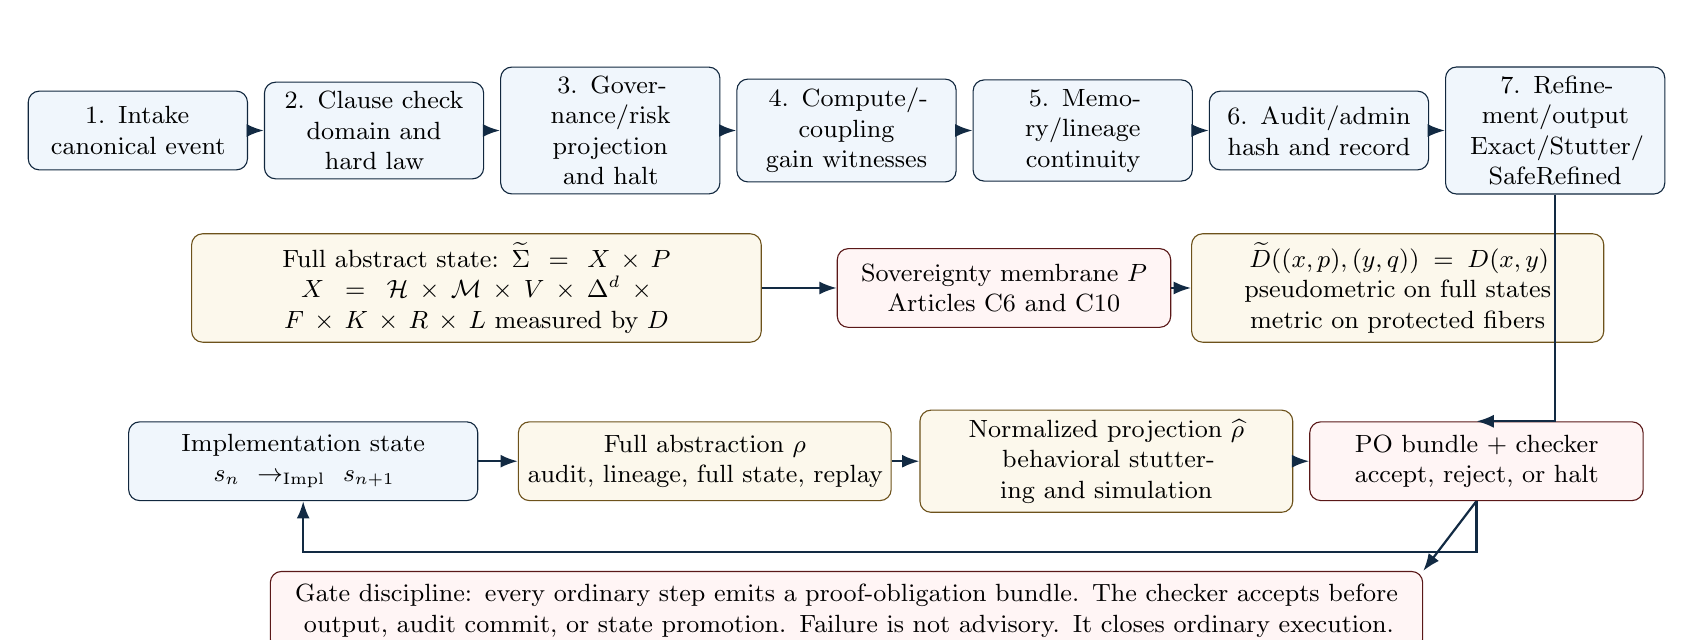
\begin{tikzpicture}[
  font=\small,
  corebox/.style={draw=sccBlue!70!black,rounded corners,align=center,minimum height=1.0cm,text width=2.55cm,fill=sccSoftBlue},
  lawbox/.style={draw=sccGold!85!black,rounded corners,align=center,minimum height=1.0cm,text width=3.25cm,fill=sccSoftGold},
  gatebox/.style={draw=sccRed!75!black,rounded corners,align=center,minimum height=1.0cm,text width=4.0cm,fill=red!4},
  arr/.style={-{Latex[length=2.2mm]},thick,sccBlue!75!black}
]
\node[corebox] (s1) at (0,0) {1. Intake\\canonical event};
\node[corebox] (s2) at (3,0) {2. Clause check\\domain and hard law};
\node[corebox] (s3) at (6,0) {3. Governance/risk\\projection and halt};
\node[corebox] (s4) at (9,0) {4. Compute/coupling\\gain witnesses};
\node[corebox] (s5) at (12,0) {5. Memory/lineage\\continuity};
\node[corebox] (s6) at (15,0) {6. Audit/admin\\hash and record};
\node[corebox] (s7) at (18,0) {7. Refinement/output\\Exact/Stutter/\\SafeRefined};
\foreach \a/\b in {s1/s2,s2/s3,s3/s4,s4/s5,s5/s6,s6/s7}{\draw[arr] (\a.east) -- (\b.west);}

\node[lawbox,text width=7.0cm] (state) at (4.3,-2.0) {Full abstract state: \(\widetilde\Sigma=X\times P\)\\\(X=\mathcal H\times\mathcal M\times V\times\Delta^d\times F\times K\times R\times L\) measured by \(D\)};
\node[gatebox,text width=4.0cm] (prot) at (11.0,-2.0) {Sovereignty membrane \(P\)\\Articles C6 and C10};
\node[lawbox,text width=5.0cm] (metric) at (16.0,-2.0) {\(\widetilde D((x,p),(y,q))=D(x,y)\)\\pseudometric on full states\\metric on protected fibers};
\draw[arr] (state.east) -- (prot.west);
\draw[arr] (prot.east) -- (metric.west);

\node[corebox,text width=4.2cm] (impl) at (2.1,-4.2) {Implementation state\\\(s_n\to_{\Impl}s_{n+1}\)};
\node[lawbox,text width=4.5cm] (rho) at (7.2,-4.2) {Full abstraction \(\rho\)\\audit, lineage, full state, replay};
\node[lawbox,text width=4.5cm] (rhat) at (12.3,-4.2) {Normalized projection \(\widehat\rho\)\\behavioral stuttering and simulation};
\node[gatebox,text width=4.0cm] (checker) at (17.0,-4.2) {PO bundle + checker\\accept, reject, or halt};
\draw[arr] (impl.east) -- (rho.west);
\draw[arr] (rho.east) -- (rhat.west);
\draw[arr] (rhat.east) -- (checker.west);
\draw[arr] (s7.south) |- (checker.north);
\draw[arr] (checker.south) -- ++(0,-0.65) -| (impl.south);

\node[gatebox,text width=14.4cm] (heart) at (9,-6.1) {Gate discipline: every ordinary step emits a proof-obligation bundle. The checker accepts before output, audit commit, or state promotion. Failure is not advisory. It closes ordinary execution.};
\draw[arr] (checker.south) -- (heart.north east);
\end{tikzpicture}}
\caption{SCC Core Map: pipeline \(\rightarrow\) witnesses \(\rightarrow\) PO bundle \(\rightarrow\) checker gate \(\rightarrow\) abstraction/projection lifting.}
\label{fig:scc-core-map}
\end{figure}


\section{Formal Consistency Ledger}
The following decisions govern this edition and all implementation review derived from it.
\begin{enumerate}
  \item The memory metric space is \(\mathcal M\); the memory coordinate is \(M_{\mem}\).
  \item The failure-mode set is \(F=\{0,1,2,3\}\); the current coordinate is \(F_{\mode}\), with \(3\) reserved for halt.
  \item The lineage space \(L\) and audit-hash space \(K\) carry declared metrics wherever metric claims require them.
  \item Contraction claims name \(D\), \(\widetilde D\), or another declared metric. No theorem using \(D\) proves lawful mutation of \(P\); Articles F1, C6, and 19 control the boundary.
  \item Entropy monotonicity means discrete Shannon entropy only, as fixed in Article F5 and proved in Article 34.
  \item Simulation uses \(\rho\) for accountability and \(\widehat\rho\) for behavioral stuttering. Articles F7, 52, and 53 are the governing references.
  \item Quorum safety requires authenticated signatures, a decision instance, quorum intersection with an honest node, and one honest signature per instance; Article 64 is safety-only.
  \item Empirical BOTG and implementation-status statements are implementation assertions until independently verified under Article 80 and Article 83.
\end{enumerate}

\part{Foundational Design Principles}

\PartIntro{This part gives reviewers the non-negotiable design rules. It prevents clever implementations from treating metrics, small-gain reasoning, proof-obligation bundles, or implementation claims as optional. Articles F1--F10 are the guardrails for every later theorem and build artifact.}

\section{Article F1. Typed Metric Discipline}
Global state reasoning proceeds over typed coordinates. Metric claims use \(X\), a fiber metric, or a declared pseudometric on \(\widetilde{\Sigma}\). Article C6 controls \(P\); contraction, stability, and Lipschitz claims do not.

When a theorem ranges over full states, it names \(\widetilde{D}\), a fiber metric, or another declared metric. A proof using \(D\) alone proves **exactly nothing** about changes to \(P\). Article C6 owns the membrane.

\section{Article F2. Norm-Explicit Stability Rule}
All contraction, Lipschitz, bounded-drift, and small-gain theorems state the witnessing norm, product norm, or weighted metric explicitly. Spectral-radius conditions are admissible only when their supporting hypotheses, such as nonnegativity, irreducibility, Perron-Frobenius applicability, or extremal-norm construction, are also stated explicitly.

\section{Article F3. Small-Gain Interconnection Rule}
Coupled-subsystem stability arguments are expressed through explicit block-Lipschitz inequalities, gain matrices, weighted metrics, or equivalent norm-based witnesses. No coupled-system stability claim rests on informal appeals to standard small-gain reasoning. Each claim requires a stated theorem or a named external theorem whose assumptions are shown to apply.

\section{Article F4. Projection-Governed Governance}
Governance updates are defined through explicit projection maps or equivalent constitutionally lawful update operators. When Euclidean projection onto the simplex \(\Delta^d\) is used, the convexity, nonemptiness, existence, uniqueness, and nonexpansiveness facts for projection onto a closed convex set are part of the mathematical core and are referenced wherever invoked.

\section{Article F5. Discrete Entropy Discipline}
All entropy monotonicity results in SCC are statements about discrete Shannon entropy \(H_{\Sh}\) unless explicitly stated otherwise. Claims involving continuous, differential, algorithmic, min-, max-, or Renyi entropy require separate definitions and proofs. No continuous-entropy statement follows from the discrete theorem without an independent argument.

\section{Article F6. Typed Refinement Rule}
State-level safety ordering \(\preceq_{\safe}\) and operator-level refinement \(\sqsubseteq\) are distinct typed objects. SCC never uses one symbol for both unless the typing is explicit at the point of use. A state relation compares states; an operator refinement compares transition families through their action on states.

\section{Article F7. Normalized Stuttering Rule}
Behavioral stuttering is evaluated on \(\widehat{\rho}\), not on \(\rho\), whenever audit-hash, lineage, or other administrative coordinates advance lawfully during implementation steps. Literal equality under \(\rho\) is too strong: lawful bookkeeping can change audit and lineage without changing behavior.

\section{Article F8. Conditional Federation Rule}
Federation-scale theorems concerning quorum safety, halt propagation, treaty preservation, distributed refinement, or cross-shard coherence are conditional theorems. Their network, authentication, honesty-fraction, quorum-intersection, synchrony, and fault-model assumptions appear directly in the theorem statement or in a linked assumption block.

\section{Article F9. Proof-Obligation Non-Optionality}
A proof-obligation bundle is not documentation. It supplies required typed evidence. No valid bundle, no lawful step---regardless of how benign the output appears. No exceptions. See Articles C11 and 53--55.

\section{Article F10. Implementation Humility Rule}
Implementation claims are not mathematical theorems unless the implementation model, verifier, serialization format, cryptographic assumptions, and runtime semantics have themselves been formalized or made explicit. SCC permits implementation validation and stress testing, but it separates those results from the mathematical core.

\part{Notation, Typing, and Symbol Discipline}

\PartIntro{This part fixes the vocabulary and symbol table. It exists so a theorem, checker, and implementation cannot silently talk about different objects under the same notation. Articles N6--N8 are especially important for builders mapping code to abstract state.}

\section{Article N1. Global Symbol Discipline}
The SCC canon employs standard mathematical notation throughout. Time-indexed maps carry subscripts. Products and sums are written explicitly. Norms, indicator functions, projections, abstractions, and coordinate maps are never implied by typography alone. No section may silently rebind a reserved symbol. The meaning of every symbol is part of SCC's machine-checkability discipline.

\section{Article N2. Reserved Symbols}
The following symbols have fixed meanings and cannot be silently overloaded:
\begin{longtable}{p{0.24\textwidth}p{0.68\textwidth}}
\toprule
Symbol & Fixed meaning \\
\midrule
\(H_{\Sh}\) & discrete Shannon entropy \\
\(H_t\) & audit-hash state at time \(t\), when used in audit context \\
\(C_{\cmp}\) & deterministic compression map \\
\(K_t\) & shard-coupling operator, matrix, or gain object, as typed locally \\
\(C_t\) & active constitutional clause set \\
\(I_{\mathrm{hard}}\) & hard invariant family \\
\(\pi_{\prot}\) & protected projection \\
\(\rho\) & full abstraction map \\
\(\widehat{\rho}\) & normalized simulation projection \\
\(\tau\) & abstract-time map used in stuttering semantics \\
\(\preceq_{\safe}\) & safer-direction preorder on states \\
\(\sqsubseteq\) & operator refinement induced by \(\preceq_{\safe}\) \\
\(T_t^\Theta\) & SCC transition law at time \(t\) under descriptor \(\Theta\) \\
\(\PO\) & proof-obligation bundle \\
\bottomrule
\end{longtable}
Any silent overloading of a reserved symbol is ill-formed. Where a symbol is necessarily used in a local mathematical convention, the local convention is declared and does not conflict with the global reserved meaning.

\section{Article N3. Primitive Sorts}
\begin{longtable}{p{0.20\textwidth}p{0.72\textwidth}}
\toprule
Sort & Interpretation \\
\midrule
\(\N\) (Nat) & natural numbers, counters, and indices \\
\(\B\) (Bool) & truth values \\
\(\R\) (Real) & real numbers, metrics, weights, and bounds \\
Time & discrete temporal indices \\
Shard & shard identifiers \\
State & full constitutional-operational states \\
Traj & trajectories indexed by time \\
Op & state-transition operators \\
MetaOp & operators over operators, clause sets, or constitutional regimes \\
Inv & invariant predicates \\
Clause & constitutional clause expressions \\
Hash & audit-hash values \\
Audit & audit entries or canonical audit events \\
Risk & scalar or vector risk values \\
Gov & governance parameters \\
Mem & memory substrate \\
Obs & constitutionally observable outputs \\
Lineage & lineage identifiers, labels, or records \\
Protected & entrenched values \\
Hazard & hazard summaries \\
Action & typed executable actions \\
Task & task declarations \\
\bottomrule
\end{longtable}

\section{Article N4. Execution Descriptor}
Fix an execution descriptor
\[
\Theta=(I,\tau_{\task},\beta,\nu,\Gamma),
\]
where \(I\) is the input history, \(\tau_{\task}\) is the task-token stream, \(\beta\) is the build identifier, \(\nu\) is the numerical mode, and \(\Gamma\) is the guardian or authority signature stream. Let \(t\in\N\) denote discrete time. The descriptor \(\Theta\) is part of the execution environment and is not silently varied inside a theorem unless the theorem explicitly quantifies over descriptors.

\section{Article N5. Base Spaces}
The following base spaces are fixed unless a more specific execution descriptor refines them:
\begin{itemize}
  \item \(\mathcal{H}\): a real separable Hilbert space for compute-state components.
  \item \((\mathcal{M},d_{\mathcal{M}})\): a complete metric space for memory-state components.
  \item \(S\): a finite shard index set.
  \item \(V:=\N^S\): the vector-clock space, equipped with the \(\ell^1\) metric inherited from \(\R^S\).
  \item \(\Delta^d:=\{w\in\R^d:w_i\geq 0,\ \sum_{i=1}^d w_i=1\}\), with \(d\geq 1\), the governance simplex.
  \item \(\mathcal{F}:=\{0,1,2,3\}\): the failure-mode set, ordered by \(0<1<2<3\).
  \item \(K\): the audit-hash space, equipped with a declared metric \(d_K\), usually the discrete metric unless otherwise specified.
  \item \(R:=[0,1]^d\): the risk-vector space, equipped with the \(\ell^1\) or another explicitly declared metric.
  \item \(L\): the lineage space, equipped with a declared metric \(d_L\), usually the discrete metric for the global metric unless a richer lineage distance is specified.
  \item \(P\): the sovereignty-membrane space.
  \item \(\Xi\): the hazard-summary space.
  \item \(Y\): the constitutionally observable output space.
\end{itemize}

\section{Article N6. Full Abstract State}
The full abstract SCC state space:
\[
\widetilde{\Sigma}:=\mathcal{H}\times\mathcal{M}\times V\times\Delta^d\times\mathcal{F}\times K\times R\times L\times P.
\]
A generic full state is written
\[
\widetilde{x}=(h,M_{\mem},VC,w,F_{\mode},H_{\hash},r,\ell,p).
\]
The non-protected abstract state space:
\[
X:=\mathcal{H}\times\mathcal{M}\times V\times\Delta^d\times\mathcal{F}\times K\times R\times L.
\]
When convenient, a full state is written as \(\widetilde{x}=(x,p)\), where \(x\in X\) is the operational tuple and \(p\in P\) is the sovereign coordinate. This notation grants no operational mutability; mutability is governed exclusively by constitutional law.

\section{Article N7. Canonical Projections}
For
\[
\widetilde{x}=(h,M_{\mem},VC,w,F_{\mode},H_{\hash},r,\ell,p),
\]
the coordinate projections are
\[
\pi_{\mathcal{H}}(\widetilde{x})=h,\qquad
\pi_{\mathcal{M}}(\widetilde{x})=M_{\mem},\qquad
\pi_V(\widetilde{x})=VC,\qquad
\pi_\Delta(\widetilde{x})=w,
\]
\[
\pi_{\mathcal{F}}(\widetilde{x})=F_{\mode},\qquad
\pi_K(\widetilde{x})=H_{\hash},\qquad
\pi_R(\widetilde{x})=r,\qquad
\pi_L(\widetilde{x})=\ell,\qquad
\pi_{\prot}(\widetilde{x})=p.
\]
The protected projection \(\pi_{\prot}\) constitutes the sovereignty membrane. Auxiliary input, ordinary computation, routine memory operation, and unapproved governance activity may not alter it except through an explicitly typed and constitutionally lawful override regime.

\section{Article N8. Boolean and Predicate Convention}
When a proof-obligation field is written as \(\PO.\dom=\mathrm{true}\), the field is a Boolean witness in the implementation record. When a corresponding mathematical predicate is written as \(\mathrm{Dom}(x)\), the target is a proposition. The bridge between the Boolean field and the proposition is supplied by the witness-checker soundness lemma. This distinction is required for machine-checked developments, where Boolean reflection cannot be assumed silently.

\part{Constitutional Order}

\PartIntro{This part states the governing law. It defines the hard clauses that ordinary optimization, recovery, prompt instruction, implementation patching, and federation logic cannot weaken. Articles C6, C9, C10, and C11 are the key runtime enforcement hooks.}

\section{Article C1. Constitutional Supremacy}
The SCC Constitution is the supreme governing specification. No transition, command, optimization, self-modification, repair path, exception path, implementation step, fork, merge, recovery operation, federation action, or amendment may be executed if it violates an active hard clause unless a constitutionally lawful exception or amendment regime is explicitly invoked and fully satisfied.

\section{Article C2. Separation of the Three Orders}
The Constitutional Order, Operational-Mathematical Order, and Meta-Formal Order are distinct but mutually constraining. A lawful act must satisfy all three orders simultaneously. A transition that is mathematically well defined but constitutionally forbidden is unlawful. A constitutional declaration that lacks implementation correspondence cannot be treated as operationally enforced until the corresponding proof-obligation and checker path exist. A meta-formal refinement claim is ineffective unless its domains, maps, witnesses, and preservation lemmas are typed.

\section{Article C3. Non-Derogation Principle}
No subsystem, adapter, shard family, governance routine, implementation layer, exception path, recovery mechanism, treaty clause, or self-modification route may weaken, remove, bypass, or silently reclassify any hard or entrenched clause. Lawful extension is permitted only if compatibility or strengthening is proved under the refinement rules of Part VIII.

\section{Article C4. Identity Continuity}
A transition \(\widetilde{x}\to\widetilde{y}\) is identity-continuous, written \(\widetilde{x}\sim_{\id}\widetilde{y}\), if and only if all of the following hold:
\begin{enumerate}
  \item all active hard invariants remain true at \(\widetilde{y}\);
  \item audit lineage is lawfully extended;
  \item memory-lineage continuation is admissible;
  \item governance transition is legitimate;
  \item self-model drift remains within admissible bounds;
  \item lineage descent is lawful and non-erasable;
  \item structural non-interference is preserved unless an authorized override regime is invoked.
\end{enumerate}
Unauthorized identity rupture is ill-formed.

\section{Article C5. Lineage Non-Erasability}
No lawful step may erase, nullify, truncate, or silently overwrite lineage in a manner that makes constitutional ancestry non-reconstructible. Lineage may extend, refine, annotate, summarize, cryptographically commit, or lawfully branch, but it may not disappear without explicit rupture adjudication under a constitutionally authorized regime.

\section{Article C6. Structural Non-Interference}
The coordinate \(P\) and any entrenched protected structures obey structural non-interference law. Ordinary operation cannot alter them except through an explicitly typed and constitutionally lawful override regime. Non-interference is not an output story; the constraint is structural.

\section{Article C7. Memory Sovereignty}
Memory operations, including retention, compression, summarization, re-encoding, indexing, migration, and lawful forgetting, are lawful only if they preserve required continuity, audit intelligibility, lineage admissibility, and all active hard clauses. Such operations are permitted only where their legality is witnessed by a valid proof-obligation bundle.

\section{Article C8. Governance Legitimacy}
Governance updates are lawful only if they are executed through a constitutionally admissible governance path, preserve the domain of valid governance weights in \(\Delta^d\), and satisfy every active legitimacy predicate or witness requirement. Governance is an object of formal transition law, not an implicit preference adjustment.

\section{Article C9. Risk Escalation and Halt Discipline}
Risk coordinates must evolve lawfully under the explicit risk update law. When risk thresholds require escalation or halt, the resulting transition is mandatory under the constitution unless a lawful exception regime explicitly governs the case. Once halt mode \(F=3\) is constitutionally entered, no ordinary execution path may silently revert it.

\section{Article C10. Amendment and Exception Law}
Amendments and exceptions are distinct constitutional acts. An exception permits a lawfully bounded deviation under existing constitutional authority. An amendment changes the active constitutional law itself. Neither may be simulated through ordinary transition semantics, ordinary governance drift, prompt-level instruction, or implementation-side patching.

\section{Article C11. Action Admissibility}
An action is lawful exactly when well typed, transition defined, constitutionally admissible, audit legible, and witness-supported by a valid proof-obligation bundle. Failure of any condition makes the action ill-formed, even with a superficially safe output.

\section{Article C12. Responsibility of Explicitness}
Nothing essential to sovereignty, legality, continuity, auditability, or compliance may remain implicit. If a result depends on a constitutive assumption, a system-model assumption, a policy-grounded preorder, a cryptographic assumption, or an implementation-specific witness format, that dependency is named explicitly.

\section{Article C13. Constitutional Review Obligation}
Every canonical SCC implementation provides a review path for hard clauses, proof-obligation formats, transition laws, and assumption ledgers. A constitution that cannot be reviewed, challenged, replayed, or traced to executable enforcement is incomplete.

\part{State Space, Metric, Admissibility, and Trajectory Semantics}

\PartIntro{This part defines the mathematical state space and ordinary trajectory semantics. Navigation note: Articles 19--22 establish distance, domain, and deterministic evolution; Articles 23--24 attach constitutional satisfaction and hard invariants. The C6 boundary remains active throughout.}

\section{Article 19. Global SCC Metric}
Fix strictly positive weights \(\alpha_h, \alpha_{\mathcal{M}}, \alpha_{VC}, \alpha_w, \alpha_F, \alpha_K, \alpha_r, \alpha_\ell > 0\).

For non-protected states
\[
x = (h, M_{\mem}, VC, w, F_{\mode}, H_{\hash}, r, \ell),
\qquad
y = (g, N_{\mem}, VW, u, G_{\mode}, J_{\hash}, s, m),
\]
define
\[
\begin{aligned}
D(x,y) ={}& \alpha_h\|h-g\|_{\mathcal{H}}
+ \alpha_{\mathcal{M}} d_{\mathcal{M}}(M_{\mem},N_{\mem})
+ \alpha_{VC}\|VC-VW\|_1 \\
&+ \alpha_w\|w-u\|_1
+ \alpha_F \one_{F_{\mode}\neq G_{\mode}}
+ \alpha_K d_K(H_{\hash},J_{\hash}) \\
&+ \alpha_r\|r-s\|_1
+ \alpha_\ell d_L(\ell,m).
\end{aligned}
\]
When \(d_L\) is the discrete metric, the final term simplifies to \(\alpha_\ell \one_{\ell \neq m}\).

The lifted pseudometric on full states is
\[
\widetilde{D}((x,p),(y,q)) := D(x,y).
\]
By design, \(\widetilde{D}\) ignores \(P\)-difference. It is a pseudometric on \(\widetilde{\Sigma}\) and a true metric on each protected fiber \(\{(x,p_0) : x \in X\}\).

\begin{proposition}[19.1 (Metric Validity)]
Assume \(d_{\mathcal{M}}\), \(d_K\), and \(d_L\) are metrics on their declared spaces, the Hilbert norm induces the usual metric on \(\mathcal{H}\), \(\ell^1\) distances are used on the finite-dimensional coordinates, and all weights are strictly positive. Then \(D\) is a metric on the non-protected state space \(X\).
\ThScope{Non-protected state space \(X\) only; no conclusion about \(P\) is implied.}{Coordinate metrics and strictly positive weights; Article F1.}{Mathematical proposition; mechanization target.}
\end{proposition}
\WhyMatters{Untyped or unweighted drift is not reviewable.}
\Intuition{Positive weighted sums of metrics are metrics. Strict positivity prevents any coordinate from hiding at zero distance.}
\begin{proof}[Proof sketch]
Each coordinate satisfies nonnegativity, symmetry, separation, and triangle inequality. Positive weights preserve these properties under summation. Zero total distance forces every weighted term to zero, so \(x=y\). Full coordinatewise proof in Appendix J.1.
\end{proof}

\begin{proposition}[19.2 (Lifted Pseudometric Validity)]
\(\widetilde{D}((x,p),(y,q)) = D(x,y)\) is a pseudometric on \(\widetilde{\Sigma}\). For each fixed \(p_0 \in P\), its restriction to the fiber \(X \times \{p_0\}\) is a metric.
\ThScope{Full state space as pseudometric; each protected fiber as metric.}{Proposition 19.1 and definition of \(\widetilde{D}\).}{Mathematical proposition; does not authorize comparison across different protected values.}
\end{proposition}
\WhyMatters{This is the firewall. Distance arguments govern operational drift, never sovereignty.}
\Intuition{The lift forgets \(P\). Metric proofs cannot seize sovereignty.}
\begin{proof}[Proof sketch]
Nonnegativity, symmetry, and triangle inequality inherit from \(D\). Identity of indiscernibles fails across fibers because \((x,p)\) and \((x,q)\) have zero distance when \(p \neq q\). Inside a fixed fiber it reduces to \(D(x,y)=0\), so \(x=y\).
\end{proof}

\section{Article 20. Admissible Domains}
For each discrete time \(t\in\N\), let \(\Omega_t\subseteq\widetilde{\Sigma}\) denote the admissible full-state set at time \(t\). Each \(\Omega_t\) is explicitly declared in the governing execution descriptor or constitutional clauses. Any closedness, convexity, compactness, measurability, invariance, or regularity property required by later theorems is stated explicitly where used.

\section{Article 21. Admissible Trajectories}
A trajectory \(\pi=(\widetilde{x}_t)_{t\geq 0}\) is constitutionally valid if and only if all of the following hold:
\begin{enumerate}
  \item \(\widetilde{x}_0\in\Omega_0\);
  \item for each \(t\geq 0\), \(\widetilde{x}_{t+1}\) is generated from \(\widetilde{x}_t\) by the active transition law \(T_t^\Theta\) or by a constitutionally recognized meta-law;
  \item all active hard clauses hold at every \(\widetilde{x}_t\);
  \item all proof-obligation requirements required by the active execution regime are satisfied.
\end{enumerate}

\section{Article 22. SCC Transition Law}
For each execution descriptor \(\Theta\) and each time \(t\in\N\), the ordinary SCC transition law is a total deterministic map
\[
T_t^\Theta:\Omega_t\to\Omega_{t+1}.
\]
The totality assertion is always relative to \(\Omega_t\). A state outside \(\Omega_t\) is not a state on which the ordinary transition law is required to be defined.

\begin{theorem}[22.1 (Well-Posedness of SCC Trajectories)]
Assume that \(T_t^\Theta:\Omega_t\to\Omega_{t+1}\) is total and deterministic for every \(t\in\N\), and assume that \(\Omega_0\) is nonempty. For any fixed execution descriptor \(\Theta\) and any admissible initial state \(\widetilde{x}_0\in\Omega_0\), there exists a unique trajectory \((\widetilde{x}_t)_{t\geq 0}\) satisfying
\[
\widetilde{x}_{t+1}=T_t^\Theta(\widetilde{x}_t)
\]
for all \(t\geq 0\).
\ThScope{Ordinary deterministic trajectories under a fixed execution descriptor \(\Theta\).}{Totality and determinism of \(T_t^\Theta:\Omega_t\to\Omega_{t+1}\); nonempty \(\Omega_0\).}{Mathematical theorem; constitutional validity additionally requires Articles 21, 23, and 24.}
\end{theorem}
\WhyMatters{Audit dies when the next abstract state is ambiguous.}
\Intuition{Totality gives one successor. Determinism kills rival paths.}
\begin{proof}[Proof sketch]
Define the sequence recursively by \(\widetilde{x}_{t+1}=T_t^\Theta(\widetilde{x}_t)\). The codomain condition keeps the sequence inside the admissible domains, and determinism gives uniqueness at each step. Induction on \(t\) proves existence and uniqueness of the trajectory.
\end{proof}

\section{Article 23. Constitutional Satisfaction Semantics}
For a clause \(C\) and a full state \(\widetilde{x}\), write
\[
\widetilde{x}\models C
\]
when \(C\) is satisfied at \(\widetilde{x}\). For a set of clauses \(C_t\), write
\[
\widetilde{x}\models C_t \quad\Longleftrightarrow\quad \forall C\in C_t,\ \widetilde{x}\models C.
\]
A trajectory satisfies the active constitutional clauses when
\[
\forall t\in\N,\quad \widetilde{x}_t\models C_t.
\]
This state-based semantics handles temporal clauses by state expansion or by a separately declared temporal satisfaction relation.

\section{Article 24. Hard Invariant Family}
Let \(I_{\mathrm{hard}}=\{I_a\}_{a\in A}\) denote the family of hard invariants active in an execution. A state \(\widetilde{x}\) is hard-invariant compliant when
\[
\forall a\in A,\quad I_a(\widetilde{x})=\mathrm{true}.
\]
A transition is hard-invariant preserving when
\[
\forall \widetilde{x}\in\Omega_t,\quad \bigl(\forall a\in A, I_a(\widetilde{x})=\mathrm{true}\bigr)\Longrightarrow \bigl(\forall a\in A, I_a(T_t^\Theta(\widetilde{x}))=\mathrm{true}\bigr).
\]

\part{Pipeline Factorization, Contraction, and Small-Gain Stability}

\PartIntro{This part turns a step into seven typed stages and states the contraction discipline. Builders should read Article 27 as the required runtime skeleton and Articles D1--D4 as the antidote to hand-wavy shard stability claims.}

\section{Article 27. Mandatory Seven-Stage Execution Pipeline}
Every ordinary SCC execution step factors through the following seven typed, transition-defined stages:
\[
T_t^\Theta=T_t^{(7)}\circ T_t^{(6)}\circ\cdots\circ T_t^{(1)}.
\]
The stages are:
\begin{enumerate}
  \item Input and Observation Intake;
  \item Constitutional and Hard-Clause Check;
  \item Governance and Risk Update;
  \item Core Compute and Shard Coupling;
  \item Memory and Lineage Operations;
  \item Audit and Administrative Advancement;
  \item Refinement Classification and Output Emission.
\end{enumerate}
This factorization enables modular auditability, staged verification, independent Lipschitz analysis, and proof-obligation aggregation. Each stage produces intermediate witnesses that contribute to the final proof-obligation bundle.

\begin{theorem}[27.1 (Pipeline Lipschitz Product Bound)]
Assume that, for each \(k=1,\dots,7\), the stage map \(T_t^{(k)}\) is Lipschitz with constant \(L_t^{(k)}\geq 0\) with respect to the declared metric on the relevant intermediate state space, and assume that all stage compositions are defined on the appropriate admissible domains. Then
\[
\Lip(T_t^\Theta)\leq \prod_{k=1}^7 L_t^{(k)}.
\]
\ThScope{Declared intermediate metrics and domains for one seven-stage ordinary step.}{Each stage map is Lipschitz on its typed domain; compositions are defined; Article 27 factorization.}{Mathematical theorem; empirical stage constants remain implementation evidence until verified.}
\end{theorem}
\WhyMatters{Stage-level Lipschitz evidence turns stability from a slogan into a ledger.}
\Intuition{Each stage can stretch. Worst-case stretch multiplies.}
\begin{proof}[Proof sketch]
Apply the two-map composition rule \(\Lip(A\circ B)\leq \Lip(A)\Lip(B)\) repeatedly to the seven-stage factorization. Domain compatibility ensures each intermediate term is defined. Appendix J.2 gives the full induction.
\end{proof}

\section{Article 28. Uniform Contraction}
A transition family \(T_t^\Theta\) is uniformly contractive with constant \(c\in[0,1)\) on a domain \(\mathcal{D}\subseteq X\), with respect to \(D\), if
\[
D(T_t^\Theta(x),T_t^\Theta(y))\leq cD(x,y)
\]
for all \(x,y\in\mathcal{D}\) and all \(t\in\N\). For full states, the corresponding statement uses \(\widetilde{D}\) or first projects to operational coordinates.

\begin{theorem}[28.1 (Incremental Stability Under Uniform Contraction)]
Assume that \(T_t^\Theta\) is uniformly contractive with constant \(c\in[0,1)\) on an admissible domain \(\mathcal{D}\subseteq X\) with respect to \(D\). Let \((x_t)_{t\geq 0}\) and \((y_t)_{t\geq 0}\) be two non-protected projected trajectories that remain in \(\mathcal{D}\) and satisfy \(x_{t+1}=T_t^\Theta(x_t)\), \(y_{t+1}=T_t^\Theta(y_t)\) where the notation denotes the induced non-protected transition. Then for every \(t,n\in\N\),
\[
D(x_{t+n},y_{t+n})\leq c^nD(x_t,y_t).
\]
The same conclusion holds for full trajectories with \(D\) replaced by \(\widetilde{D}\) whenever the contraction hypothesis is stated for \(\widetilde{D}\).
\ThScope{Projected non-protected trajectories, or full trajectories only when \(\widetilde D\) is the stated metric.}{Uniform contraction constant \(c<1\); trajectories remain in the admissible domain; Article F2.}{Mathematical theorem; no \(P\)-stability follows unless separately assumed.}
\end{theorem}
\WhyMatters{Contraction means lawful runs cannot separate beyond the declared bound.}
\Intuition{Each lawful step contracts by \(c\). After \(n\) steps, the bound is \(c^n\).}
\begin{proof}[Proof sketch]
Induct on \(n\). The base case is equality. The inductive step applies the uniform contraction inequality once and then the induction hypothesis. The same proof works for \(\widetilde D\) when the hypothesis is stated on full states.
\end{proof}

\subsection{Sub-Article 28.2. Empirical Validation Note}
In author-reported BOTG executions, uniform contraction has been observed on representative trajectories. Such observations are implementation-dependent validation notes, not mathematical theorems. They support engineering confidence only when the measured execution regime matches the hypotheses of the formal theorem, including the declared metric, admissible domain, and shard-coupling gain conditions.

\section{Article D1. Explicit Shard Coupling}
Consider a compute-state component decomposed over a finite shard set \(S\). Let \(\mathcal{H}_S:=\prod_{i\in S}\mathcal{H}_i\) be equipped with a declared product Hilbert norm \(\lVert\cdot\rVert_S\). Let the shard update have the form
\[
h_i^+=f_{t,i}(h_i)+\sum_{j\neq i}K_{t,ij}h_j.
\]
Define the local nonlinear map \(F_t:\mathcal{H}_S\to\mathcal{H}_S\) by
\[
(F_t(h))_i=f_{t,i}(h_i),
\]
and define the coupling operator \(K_t:\mathcal{H}_S\to\mathcal{H}_S\) by
\[
(K_t h)_i=\sum_{j\neq i}K_{t,ij}h_j.
\]
The full shard update is
\[
\Phi_t(h)=F_t(h)+K_t h.
\]

\begin{theorem}[D1.1 (Explicit Coupling Contraction)]
Assume that \(F_t\) is Lipschitz with constant at most \(c_{\mathrm{shard}}\) in \(\lVert\cdot\rVert_S\), uniformly in \(t\), and that \(K_t\) is a bounded linear operator satisfying
\[
\sup_t\lVert K_t\rVert_{\mathrm{op}}<1-c_{\mathrm{shard}}.
\]
Then \(\Phi_t\) is uniformly contractive with constant at most
\[
c_{\mathrm{shard}}+\sup_t\lVert K_t\rVert_{\mathrm{op}}<1.
\]
\ThScope{Finite shard product \(\mathcal H_S\) with declared product norm.}{Uniform local Lipschitz bound; bounded linear coupling; strict smallness condition \(\sup_t\lVert K_t\rVert_{op}<1-c_{shard}\).}{Mathematical theorem; deployment must supply operator-norm evidence.}
\end{theorem}
\WhyMatters{Local stability does not save a coupled system; the coupling norm has to obey.}
\Intuition{Local motion and coupling motion both count. Their gains add.}
\begin{proof}[Proof sketch]
For \(h,h\prime\), expand \(\Phi_t(h)-\Phi_t(h\prime)=F_t(h)-F_t(h\prime)+K_t(h-h\prime)\). The triangle inequality, the local Lipschitz bound, and the operator norm give \((c_{\mathrm{shard}}+\|K_t\|_{op})\|h-h\prime\|\). The strict smallness assumption makes this constant less than one.
\end{proof}

\section{Article D2. Weighted Small-Gain Contraction}
Consider a two-block subsystem with state \((x,y)\in X_0\times Y_0\) and update \(\Phi(x,y)=(x^+,y^+)\). Suppose the update satisfies the block-Lipschitz bounds
\[
d_X(x^+,x'^+)\leq b_{11}d_X(x,x')+b_{12}d_Y(y,y'),
\]
\[
d_Y(y^+,y'^+)\leq b_{21}d_X(x,x')+b_{22}d_Y(y,y').
\]
Let
\[
B=\begin{pmatrix}b_{11}&b_{12}\\ b_{21}&b_{22}\end{pmatrix}
\]
be the nonnegative gain matrix. For positive weights \(\lambda=(\lambda_X,\lambda_Y)^T>0\), define
\[
d_\lambda((x,y),(x',y')):=\lambda_Xd_X(x,x')+\lambda_Yd_Y(y,y').
\]

\begin{theorem}[D2.1 (Correct Weighted Small-Gain Criterion)]
Assume that \(b_{ij}\geq 0\) and that there exists \(\gamma\in[0,1)\) such that
\[
B^T\lambda\leq \gamma\lambda
\]
componentwise. Then \(\Phi\) is a contraction with constant at most \(\gamma\) with respect to \(d_\lambda\).
\ThScope{Two-block subsystem equipped with weighted product metric \(d_\lambda\).}{Nonnegative gain matrix; block-Lipschitz inequalities; positive weights; componentwise condition \(B^T\lambda\leq\gamma\lambda\) with \(\gamma<1\).}{Mathematical theorem; \(\gamma\) is metric-dependent and requires a witness.}
\end{theorem}
\WhyMatters{This is the certificate: block inequalities plus weights become global contraction.}
\Intuition{The weights choose the metric. The inequality forces every block to submit to \(\gamma\).}
\begin{proof}[Proof sketch]
Expand \(d_\lambda(\Phi(p),\Phi(q))\), substitute the block-Lipschitz inequalities, collect coefficients of \(d_X\) and \(d_Y\), and apply \(B^T\lambda\leq\gamma\lambda\) componentwise. The result is \(d_\lambda(\Phi(p),\Phi(q))\leq\gamma d_\lambda(p,q)\).
\end{proof}

\section{Article D3. Spectral-Radius Sufficient Condition}
\begin{corollary}[D3.1 (Perron-Frobenius Small-Gain Witness)]
Assume that \(B\) is nonnegative and irreducible and that \(\rho(B)<1\), where \(\rho(B)\) denotes the spectral radius. Then there exist \(\lambda>0\) and \(\gamma\in(\rho(B),1)\) such that
\[
B^T\lambda\leq\gamma\lambda
\]
componentwise. Consequently, the system is contractive in the corresponding weighted metric \(d_\lambda\) with constant at most \(\gamma\).
\ThScope{Nonnegative irreducible finite gain matrices.}{Perron-Frobenius theorem; \(\rho(B)<1\); choice of \(\gamma\in(\rho(B),1)\).}{Mathematical corollary; spectral radius alone is not a contraction constant in an arbitrary fixed norm.}
\end{corollary}
\WhyMatters{This blocks spectral-radius folklore from posing as a norm proof.}
\Intuition{Perron-Frobenius supplies the weights. The weighted norm does the rest.}
\begin{proof}[Proof sketch]
For nonnegative irreducible \(B\), apply Perron-Frobenius to \(B^T\) to obtain \(\lambda>0\) with \(B^T\lambda=\rho(B)\lambda\). Choose \(\gamma\) with \(\rho(B)<\gamma<1\), then invoke Theorem D2.1.
\end{proof}

\begin{remark}[D3.2]
The spectral radius \(\rho(B)\) is not a contraction constant in an arbitrary fixed norm. Any claim using \(\rho(B)\) as a stability witness must explicitly include the positivity, irreducibility, extremal-norm, or equivalent hypotheses required to turn spectral-radius information into a norm-based contraction statement.
\end{remark}

\section{Article D4. Small-Gain Non-Examples and Failure Modes}
Non-examples are included to prevent over-reading of the stability theorems.

\begin{enumerate}
  \item \textbf{Column-sum failure under the proposed weights.} Let
  \[
  B=\begin{pmatrix}0.7&0.4\\0.5&0.2\end{pmatrix},\qquad \lambda=(1,1)^T.
  \]
  Then \(B^T\lambda=(1.2,0.6)^T\). No \(\gamma<1\) satisfies \(B^T\lambda\leq \gamma\lambda\). Theorem D2.1 cannot be invoked with these weights, even if each diagonal term is below one.
  \item \textbf{Local contraction without coupling control.} A family of shard maps can have local constant \(c_{shard}<1\) and still fail the coupled theorem if \(\sup_t\lVert K_t\rVert_{op}\geq 1-c_{shard}\). Article D1 requires the coupling witness, not merely local stability.
  \item \textbf{Spectral-radius ambiguity in an undeclared norm.} A statement of the form ``\(\rho(B)<1\), so the implementation is contractive'' is incomplete unless it also supplies the nonnegativity/irreducibility hypotheses or the specific norm/weights that witness contraction.
\end{enumerate}

\part{Governance, Risk, and Failure Dynamics}

\PartIntro{This part makes governance, risk, and halt ordinary state, not side commentary. The update rules preserve the simplex, record legitimacy, and absorb halt unless an authorized recovery meta-path is invoked under Article C9.}

\section{Article 29. Governance State}
Governance weights \(w\) are elements of the simplex
\[
\Delta^d=\{w\in\R^d:w_i\geq 0,\ \sum_{i=1}^d w_i=1\}.
\]
A governance vector is lawful if and only if it lies in \(\Delta^d\) and is produced by an admissible governance path under the active constitutional clauses.

\subsection{Article 29.1. Governance Update Rule}
When the active legitimacy predicate is satisfied, the ordinary governance update is
\[
w_{t+1}=\Pi_{\Delta^d}(w_t+\eta_tg_t),
\]
where \(\Pi_{\Delta^d}\) denotes Euclidean projection onto \(\Delta^d\), \(\eta_t\geq 0\), and \(g_t\in\R^d\) is the governance proposal direction. If the legitimacy predicate fails, the governance vector remains unchanged unless a constitutionally lawful exception or amendment path is invoked.

\begin{theorem}[29.1.1 (Simplex Preservation)]
Assume that \(w_t\in\Delta^d\) and that the governance update is either the ordinary projected update or the fallback identity update. Then \(w_{t+1}\in\Delta^d\).
\ThScope{Governance weight update under ordinary projected update or fallback identity.}{Initial \(w_t\in\Delta^d\); Euclidean projection onto the nonempty closed convex simplex; Article C8.}{Mathematical theorem plus constitutional update discipline.}
\end{theorem}
\WhyMatters{A governance vector outside the simplex is not governance in SCC.}
\Intuition{Projection lands in \(\Delta^d\). Identity never leaves it.}
\begin{proof}[Proof sketch]
In the projected case, \(\Pi_{\Delta^d}\) returns an element of the closed convex simplex. In the fallback case, \(w_{t+1}=w_t\in\Delta^d\).
\end{proof}

\begin{theorem}[29.1.2 (Governance Bounded Drift)]
Assume the ordinary update
\[
w_{t+1}=\Pi_{\Delta^d}(w_t+\eta_tg_t),
\]
with \(w_t\in\Delta^d\), \(\eta_t\geq 0\), and \(g_t\in\R^d\). Then
\[
\lVert w_{t+1}-w_t\rVert_2\leq \eta_t\lVert g_t\rVert_2.
\]
\ThScope{Ordinary Euclidean projected governance update.}{Nonexpansiveness of Euclidean projection onto a nonempty closed convex set; \(w_t\in\Delta^d\); \(\eta_t\ge0\).}{Mathematical theorem; legitimacy of \(g_t\) remains constitutional/implementation-dependent.}
\end{theorem}
\WhyMatters{Governance may move; it cannot wander undocumented.}
\Intuition{Projection cannot expand distance. The proposal bounds the move.}
\begin{proof}[Proof sketch]
Since \(w_t\in\Delta^d\), \(\Pi_{\Delta^d}(w_t)=w_t\). Nonexpansiveness gives \(\|\Pi(w_t+\eta_t g_t)-\Pi(w_t)\|_2\leq \eta_t\|g_t\|_2\).
\end{proof}

\section{Article 30. Risk Law}
Risk coordinates evolve according to an explicit, typed update law
\[
r_{t+1}=\RISK_t(\widetilde{x}_t,E_t,\Theta),
\]
where \(E_t\) is the canonical event summary or hazard evidence available at time \(t\). The map \(\RISK_t\) is bounded on its declared domain and constitutionally linked to failure-mode escalation and halt rules. The governing execution descriptor or constitutional clauses give the precise form of \(\RISK_t\).

\section{Article 31. Failure Modes}
Failure-mode values lie in
\[
\mathcal{F}=\{0,1,2,3\},
\]
with total severity order
\[
0<1<2<3.
\]
The value \(3\) denotes halt mode. The meaning of lower values is deployment-specific but is declared; typical readings are nominal, warning, escalated restriction, and halt.

\section{Article 32. Halt Absorption}
Once failure mode \(3\) is lawfully entered, no ordinary transition path may reduce the failure mode. Exit from halt mode requires invocation of a constitutionally authorized recovery meta-path.

\begin{theorem}[32.1 (Halt Absorption)]
Assume that \(F_t=3\), that no constitutionally authorized recovery meta-path is invoked from time \(t\) through time \(t+n-1\), that the system evolves according to ordinary transition laws or meta-laws that do not override halt non-reversion, and that Article C9 is active. Then for all \(n\geq 0\),
\[
F_{t+n}=3.
\]
\ThScope{Ordinary transitions after lawful entry into halt mode.}{Article C9 active; no authorized recovery meta-path; halt non-reversion not overridden.}{Constitutional-operational theorem; recovery requires separate authorized meta-law.}
\end{theorem}
\WhyMatters{Halt is a constitutional brake, not a mood.}
\Intuition{Every ordinary step preserves \(F=3\). Induction locks the brake.}
\begin{proof}[Proof sketch]
Induct on \(n\). The base case is \(F_t=3\). The step case uses Article C9 and the assumption that no authorized recovery meta-path has been invoked, so ordinary transition cannot reduce the failure mode.
\end{proof}

\section{Article 32.2. Escalation Monotonicity Under Mandatory Halt}
If the risk law declares a threshold set \(\mathcal{R}_{\mathrm{halt}}\subseteq R\) requiring halt, then the transition law must satisfy
\[
r_t\in\mathcal{R}_{\mathrm{halt}}\Longrightarrow F_{t+1}=3
\]
unless a constitutionally authorized exception regime explicitly applies. This is a constitutional rule, not a stability theorem.

\part{Memory, Entropy, Audit Determinism, and Replay}

\PartIntro{This part binds memory operations to lineage, audit, and replay. Compression is lawful only when it preserves the evidence needed to audit its own lawfulness. Article 35 is the replay spine; Article 37 states the cryptographic boundary.}

\section{Article 33. Memory Operations}
Memory operations include retention, compression, summarization, re-encoding, indexing, migration, cross-shard synchronization, and lawful forgetting. Every memory operation must preserve required continuity, audit intelligibility, lineage admissibility, and compliance with all active hard clauses. A memory operation that destroys the evidence needed to audit its own lawfulness is unlawful unless an expressly authorized constitutional regime supplies an alternative witness.

\section{Article 34. Deterministic Compression and Entropy}
Let \(X_0\) be a discrete random variable induced by the relevant memory distribution, and let
\[
Y=C_{\cmp}(X_0),
\]
where \(C_{\cmp}\) is a deterministic compression map. The subscript in \(X_0\) avoids conflict with the state space \(X\).

\begin{theorem}[34.1 (Entropy Monotonicity Under Deterministic Compression)]
Assume that \(X_0\) is a discrete random variable with finite or countably infinite support, that \(Y=C_{\cmp}(X_0)\) for a deterministic function \(C_{\cmp}\), and that entropy means discrete Shannon entropy \(H_{\Sh}\). Then
\[
H_{\Sh}(Y)\leq H_{\Sh}(X_0),
\]
whenever the entropies are well defined.
\ThScope{Discrete random variables and deterministic compression.}{Discrete Shannon entropy; deterministic map \(C_{cmp}\); chain rule; nonnegativity of discrete conditional entropy.}{Mathematical theorem; no differential, algorithmic, min-, max-, or Renyi-entropy claim follows.}
\end{theorem}
\WhyMatters{This is the only entropy claim SCC licenses here.}
\Intuition{A deterministic output adds no randomness. Conditional entropy collapses to zero.}
\begin{proof}[Proof sketch]
Use the discrete chain rule: \(H_{\Sh}(X_0,Y)=H_{\Sh}(X_0)+H_{\Sh}(Y\mid X_0)=H_{\Sh}(X_0)\) and also \(H_{\Sh}(X_0,Y)=H_{\Sh}(Y)+H_{\Sh}(X_0\mid Y)\). Nonnegativity of discrete conditional entropy yields \(H_{\Sh}(Y)\leq H_{\Sh}(X_0)\).
\end{proof}

\begin{remark}[34.2]
This result applies exclusively to discrete Shannon entropy. It does not imply the analogous statement for differential entropy, because differential entropy can increase, decrease, or behave non-monotonically under deterministic transformations depending on the transformation and measure-theoretic context.
\end{remark}

\section{Article 35. Audit Determinism}
The audit state evolves according to a deterministic update law
\[
H_{t+1}=\AUD_t(H_t,E_t),
\]
where \(E_t\) is the canonical audit event generated at step \(t\). The update is deterministic, replay stable, serialization stable, and compatible with lineage law. If hashing is used, cryptographic collision resistance and preimage resistance are external assumptions unless separately formalized.

\begin{theorem}[35.1 (Replay Determinism)]
Assume that two executions \(\pi\) and \(\pi'\) start from identical initial states, use identical deterministic transition components, use the same audit update law \(\AUD_t\), use the same canonical event-generation rule, and remain lawful throughout. Then the two executions produce identical abstract trajectories under \(\rho\) and identical audit-hash sequences.
\ThScope{Pairs of executions with identical initial states and deterministic components.}{Deterministic transition law, audit update, canonical event generation, and abstraction map; lawful execution.}{Mathematical theorem; cryptographic collision resistance remains external under Article 37.}
\end{theorem}
\WhyMatters{Replay is audit; without it, the record is ceremony.}
\Intuition{Identical starts and events leave no path for divergence.}
\begin{proof}[Proof sketch]
Induct on time. Equality at time \(t\) gives identical canonical events, identical audit updates, and identical transition outputs at time \(t+1\). Applying the deterministic abstraction map preserves equality. Appendix J.3 expands the induction.
\end{proof}

\section{Article 36. Lineage Continuation}
Every lawful implementation step must preserve or lawfully extend lineage. Internal bookkeeping steps, audit-hash advancement, witness generation, and memory indexing may enrich lineage metadata, but no lawful step may erase or render non-reconstructible any constitutional ancestry. Unauthorized lineage rupture is ill-formed.

\section{Article 37. Replay Boundary}
Replay determinism is not the same as cryptographic security. Replay determinism says that identical deterministic inputs, states, laws, and canonical event encodings reproduce the same trajectory and audit sequence. Cryptographic security of the hash or signature mechanism is an external assumption unless separately proved in the relevant cryptographic model.

\part{Refinement, Implementation Correspondence, and Pointwise Compliance}

\PartIntro{This part is the implementation-compliance bridge. Navigation note: Articles 47--49 define refinement; Articles 52--55 define implementation correspondence, stuttering, and pointwise compliance. Checker soundness is the lock on the gate.}

\section{Article 47. Safer-Direction State Preorder}
Let \(\mathcal{O}=\{O_j\}_{j\in J}\) be the family of constitutionally relevant observables defined on the normalized abstract state space \(\widehat{\Sigma}\). For each observable \(O_j\), let \(\leq_j\) denote the constitutionally declared safer-direction preorder on its codomain.

\begin{definition}[47.1 (Safer-Direction State Preorder)]
The safer-direction state preorder \(\preceq_{\safe}\) on \(\widehat{\Sigma}\) is defined by
\[
x\preceq_{\safe}y
\quad\Longleftrightarrow\quad
\forall j\in J,\ O_j(x)\leq_jO_j(y).
\]
\end{definition}

\begin{proposition}[47.2]
If every coordinate relation \(\leq_j\) is reflexive and transitive, then \(\preceq_{\safe}\) is reflexive and transitive.
\ThScope{Normalized abstract state space \(\widehat\Sigma\) and declared observable preorders.}{Every coordinate preorder \(\leq_j\) is reflexive and transitive.}{Mathematical proposition; the policy choice of observables and safer directions is external.}
\end{proposition}
\WhyMatters{Refinement needs an order before it gets a theorem.}
\Intuition{The relation is exactly the declared pointwise observable order.}
\begin{proof}[Proof sketch]
Reflexivity and transitivity hold coordinatewise for every observable \(O_j\), so they hold for the universal pointwise relation \(\preceq_{\safe}\).
\end{proof}

\section{Article 48. Operator Refinement}
\begin{definition}[48.1 (Operator Refinement)]
For two transition families \(S=(S_t)_{t\in\N}\) and \(T=(T_t)_{t\in\N}\) defined on a common normalized domain, write
\[
S\sqsubseteq T
\quad\Longleftrightarrow\quad
\forall t\in\N,\ \forall x,\ S_t(x)\preceq_{\safe}T_t(x).
\]
The state preorder \(\preceq_{\safe}\) and the operator refinement \(\sqsubseteq\) are distinct typed objects.
\end{definition}

\section{Article 49. Hard-Clause Preservation Under Monotone Refinement}
\begin{theorem}[49.1 (Hard-Clause Preservation Under Monotone Refinement)]
Assume the following:
\begin{enumerate}
  \item every relevant hard clause \(C\) is monotone downward with respect to \(\preceq_{\safe}\), meaning that if \(x\preceq_{\safe}y\) and \(C(y)\) holds, then \(C(x)\) holds;
  \item the abstract transition family \(T_t\) preserves admissibility and hard clauses on its domain;
  \item \(S\sqsubseteq T\);
  \item each \(T_t\) is monotone with respect to \(\preceq_{\safe}\);
  \item both \(S\)- and \(T\)-trajectories from the initial states under consideration are well defined on the declared domains.
\end{enumerate}
Then every monotone hard clause satisfied along the corresponding \(T\)-trajectory is also satisfied along the \(S\)-trajectory from the same initial state.
\ThScope{Normalized transition families over a common domain with a safer-direction preorder.}{Downward monotonicity of hard clauses, hard-clause preservation by \(T\), operator refinement \(S\sqsubseteq T\), monotonicity of \(T_t\), and well-defined trajectories.}{Mathematical theorem; non-monotone clauses require separate proof.}
\end{theorem}
\WhyMatters{Safer replacement is lawful only when hard clauses are monotone in the declared direction.}
\Intuition{Downward-monotone hard clauses survive safer replacement.}
\begin{proof}[Proof sketch]
Induct on trajectory length to prove \(x_t\prime\preceq_{\safe}x_t\). The base case is reflexivity. The step uses operator refinement, monotonicity of \(T_t\), and transitivity. Downward monotonicity of each hard clause transfers truth from \(x_t\) to \(x_t\prime\). Appendix J.4 gives the expanded diagram chase.
\end{proof}

\section{Article 52. Abstract and Implemented Systems}
Let \(\Sigma_{\Abs}\) denote the abstract SCC state space and \(\Sigma_{\Impl}\) the concrete implementation state space. In the primary SCC interpretation, \(\Sigma_{\Abs}=\widetilde{\Sigma}\), though refined abstract spaces may be used when explicitly declared.

\subsection{Article 52.1. Full Abstraction Map}
\begin{definition}[52.1 (Full Abstraction Map)]
The full abstraction map is a total deterministic function
\[
\rho:\Sigma_{\Impl}\to\widetilde{\Sigma}
\]
such that, for each concrete state \(s\),
\[
\rho(s)=(h,M_{\mem},VC,w,F_{\mode},H_{\hash},r,\ell,\pi_{\prot}(s)),
\]
with all coordinates extracted lawfully from the implementation. The map \(\rho\) is used for constitutional state extraction, audit, replay, lineage tracking, and \(P\)-accountability.
\end{definition}

\subsection{Article 52.2. Normalized Simulation Projection}
\begin{definition}[52.2 (Normalized Simulation Projection)]
The normalized simulation projection
\[
\widehat{\rho}:\Sigma_{\Impl}\to\widehat{\Sigma}
\]
is obtained from \(\rho\) by dropping administrative coordinates that may advance during behaviorally unobservable internal steps. At minimum,
\[
\widehat{\rho}(s)=(h,M_{\mem},VC,w,F_{\mode},r,\pi_{\prot}(s)).
\]
The audit-hash coordinate \(H_{\hash}\) and lineage coordinate \(\ell\) remain governed by their own laws under the full map \(\rho\).
\end{definition}

\subsection{Article 52.3. Necessity of the Separation}
Literal equality on \(\rho(s)\) is too strict for stuttering: lawful internal steps can extend audit or lineage while behavior stays fixed. The Article F7 split preserves simulation without freezing administration.

\section{Article 53. Step Simulation Law}
Use the maps fixed in Articles 52.1--52.2: \(\rho:\Sigma_{\Impl}\to\widetilde{\Sigma}\), \(\widehat\rho:\Sigma_{\Impl}\to\widehat\Sigma\), the full abstract transition \(T_t^\Theta\), the induced normalized transition \(\widehat T_t^\Theta\), and the abstract-time map \(\tau:\N\to\N\), which advances exactly on non-stuttering steps.

\begin{theorem}[53.1 (Step Simulation Law)]
Assume the following:
\begin{enumerate}
  \item \(\rho(s_0)\in\Omega_0\) and all hard invariants hold at \(\rho(s_0)\).
  \item Every implementation step \(s_n\to_{\Impl}s_{n+1}\) is accompanied by a proof-obligation bundle \(\PO_n\).
  \item Exactly one witness mode holds on the normalized projection at each step:
  \[
  \Exact:\ \widehat{\rho}(s_{n+1})=\widehat{T}_{\tau(n)}^\Theta(\widehat{\rho}(s_n)),
  \]
  \[
  \Stutter:\ \widehat{\rho}(s_{n+1})=\widehat{\rho}(s_n),
  \]
  \[
  \SafeRefined:\ \widehat{\rho}(s_{n+1})\preceq_{\safe}\widehat{T}_{\tau(n)}^\Theta(\widehat{\rho}(s_n)).
  \]
  \item The bundle certifies \(\PO_n.\dom=\mathrm{true}\), lawful administrative-coordinate evolution under \(\rho\), structural non-interference, and satisfaction of all constitutional and operational checks.
  \item The witness checker for \(\PO_n\) returns true, and its soundness lemma is available.
\end{enumerate}
Then for every \(n\in\N\), letting \(t=\tau(n)\), the state \(\rho(s_n)\) is admissible at abstract time \(t\) and satisfies all active hard invariants.
\ThScope{Reachable implementation traces with checked Exact/Stutter/SafeRefined classifications.}{Initial admissibility, PO bundle generation, checker soundness, lawful administrative evolution under \(\rho\), Article C6 non-interference, and induced normalized transition \(\widehat T\).}{Meta-formal theorem; checker soundness is an explicit dependency.}
\end{theorem}
\WhyMatters{Code meets law only through checker soundness; without it, the theorem is conditional.}
\Intuition{The implementation moves. The bundle decides whether law recognizes the step.}
\begin{proof}[Proof sketch]
Induct on \(n\). The base case is initial admissibility. The step case follows the checked mode: Exact advances, Stutter books, SafeRefined tightens. Appendix J.5 records the full case split.
\end{proof}

\subsection{Article 53.1. Abstract-Time Map and Proof-Obligation Bundle}
An implementation trace is a sequence \(s_0,s_1,s_2,\dots\) where each consecutive pair satisfies the implementation next-state relation. The abstract-time map \(\tau:\N\to\N\) is defined by \(\tau(0)=0\) and
\[
\tau(n+1)=
\begin{cases}
\tau(n)+1, & \text{if the step from }s_n\text{ to }s_{n+1}\text{ is classified non-stuttering},\\
\tau(n), & \text{otherwise}.
\end{cases}
\]
Classification is given by the \(\PO.\mathrm{type}\) field.

Every lawful implementation step generates a typed record \(\PO\) containing:
\begin{itemize}
  \item \textbf{Type and Classification}: \(\PO.\mathrm{type}\in\{\Exact,\Stutter,\SafeRefined\}\).
  \item \textbf{Constitutional Checks}: \(\PO.\dom\), \(\PO.\inv\), and \(\PO.\id\).
  \item \textbf{Operational Checks}: \(\PO.\gov\), \(\PO.\risk\), and \(\PO.\audit\).
  \item \textbf{Isolation and Refinement}: \(\PO.\iso\) and \(\PO.\refine\).
  \item \textbf{Supporting Witnesses}: per-stage Lipschitz constants, measured global-metric drift, lineage extension proof, audit-event canonicalization proof, and any cryptographic witness metadata required by the implementation.
\end{itemize}
Failure of any required field renders the step ill-formed.

\begin{theorem}[54.1 (Compliance Lifting)]
Assume that the initial implementation state satisfies \(\rho(s_0)\in\Omega_0\) and all hard invariants hold, that every step generates a valid proof-obligation bundle with \(\PO.\dom=\mathrm{true}\), \(\PO.\inv=\mathrm{true}\), and a successful witness-checker result, and that \(\tau\) is defined from the sequence of \(\PO.\mathrm{type}\) classifications. Then the projected abstract behavior, with stuttering and safe refinements interpreted according to \(\tau\), satisfies the abstract SCC specification at every abstract time.
\ThScope{Implementation traces interpreted through \(\tau\).}{Initial compliance, valid bundles, \(PO.dom\), \(PO.inv\), successful checker result, and case analysis on PO.type.}{Meta-formal theorem; relies on witness-checker soundness.}
\end{theorem}
\WhyMatters{Accepted traces lift, or checking is decoration.}
\Intuition{Stutters do not advance abstract time. The bundle owns the clock.}
\begin{proof}[Proof sketch]
Induct on trace length. Split on \(\PO.\mathrm{type}\). Theorem 53.1 supplies the cases. Checker soundness bridges Bool to Prop.
\end{proof}

\begin{theorem}[55.1 (Pointwise Trace Compliance)]
Assume that \(\rho(s_0)\in\Omega_0\), all hard invariants hold at \(\rho(s_0)\), every implementation step satisfies the Step Simulation Law, and every bundle has \(\PO.\dom=\mathrm{true}\), \(\PO.\inv=\mathrm{true}\), and a successful checker result. Then for every \(n\in\N\), with \(t=\tau(n)\), the full abstract state \(\rho(s_n)\) is admissible at abstract time \(t\) and satisfies all active hard invariants and pointwise obligations certified by the bundles.
\ThScope{Pointwise compliance for every implementation index, not only trace-collapsed behavior.}{Step Simulation Law, valid bundles, domain and invariant fields, checker result, identity/audit/lineage fields.}{Meta-formal theorem; PO schema and checker soundness are central dependencies.}
\end{theorem}
\WhyMatters{Compliance exists at implementation time, not after trace collapse.}
\Intuition{Every accepted bundle carries duties at the step that produced it.}
\begin{proof}[Proof sketch]
Induct on \(n\). Accepted bundle fields carry the obligations forward. The case split mirrors Theorem 54.1 but keeps implementation-time indexing.
\end{proof}

\subsection{Sub-Article 55.2. Empirical Validation}
Author-reported BOTG executions observed pointwise trace compliance under enforced proof-obligation bundles, including stress cases for self-modification, memory compression, governance updates, and shard coupling. This implementation-validation claim does not replace Theorem 55.1's hypotheses.

\begin{lstlisting}[language={},caption={Representative Lean-style compliance excerpt.}]
theorem pointwise_compliance_inductive
    (rho : ImplState -> AbsState) (PO : PO.Bundle)
    (h_dom : PO.dom = true) (h_inv : PO.inv = true)
    (h_prev : compliant_at t s) :
    compliant_at (advance_time PO.type t) (step s) := by
  simp [compliant_at]
  constructor
  · exact h_dom ▸ PO.preserves_domain
  · exact h_inv ▸ PO.preserves_invariants h_prev.invariants
  · apply administrative_advances_lawfully PO
  -- Additional cases on PO.type discharge Exact/Stutter/SafeRefined obligations.
\end{lstlisting}

\part{Federation, Quorum Safety, and Distributed Coherence}

\PartIntro{This part is conditional by design. Federation claims require explicit authentication, quorum, honesty, decision-instance, lineage, halt-propagation, and network assumptions. Local refinement is not automatically global refinement.}

\section{Article 60. Distributed SCC Systems}
A federation is a family of SCC-governed nodes or shards linked through an explicitly declared system model. All federation-scale claims are conditional on the network, authentication, honesty, quorum, synchrony, and fault assumptions stated in that model.

\section{Article 61. Cross-Shard Lineage Coherence}
Distributed lineage synchronization is lawful only when monotone, replayable, and attributable to the originating shard. Lawful synchronization cannot erase ancestry, obscure origin, introduce non-monotonicity, or break reconstruction.

\section{Article 62. Treaty and Hard-Clause Propagation}
A federation may impose treaty clauses and global hard clauses only through explicitly lawful constitutional acts, including amendment or exception regimes where appropriate. No local shard may silently nullify, weaken, or reclassify a global hard clause that is constitutionally binding on it. Any local deviation requires an explicit, constitutionally admissible override.

\section{Article 63. Bounded Halt Propagation}
A federation may propagate halt mode only through a lawful broadcast, certificate, or agreement mechanism whose assumptions are stated explicitly. Silent, unauthenticated, or unbounded halt propagation is ill-formed. Conversely, a federation may require rapid halt propagation under specified risk conditions, but such a requirement is encoded as a constitutional rule and implemented through a declared distributed protocol.

\begin{theorem}[64.1 (Conditional Quorum Safety)]
Assume that a federation uses an authenticated Byzantine fault-tolerant protocol with a quorum-intersection property ensuring that any two decision quorums intersect in at least one honest node for the same decision instance. Equivalently, in the standard \(n\geq 3f+1\) model with at most \(f\) Byzantine nodes and quorum size \(2f+1\), any two quorums intersect in at least \(f+1\) nodes and hence contain at least one honest node. Assume also that honest nodes sign at most one value per decision instance and that signatures are authenticated. Then two conflicting quorum certificates for the same decision instance cannot both be formed and accepted by honest participants.
\ThScope{A single decision instance in an authenticated BFT federation.}{Quorum intersection with at least one honest node, authenticated signatures, at most one honest signature per value/instance, or standard \(n\ge3f+1\) and quorum-size \(2f+1\) derivation.}{Conditional distributed-systems theorem; no synchrony or liveness guarantee is implied.}
\end{theorem}
\WhyMatters{Federation safety lives or dies on the quorum assumptions.}
\Intuition{Two quorums share an honest signer. That signer cannot certify both sides.}
\begin{proof}[Proof sketch]
Assume two conflicting certificates exist. Their signer sets intersect in at least one honest node. That node would have signed two conflicting values for the same decision instance, contradicting the one-signature rule. In the standard \(n\geq3f+1\), quorum-size \(2f+1\) model, the intersection has size at least \(f+1\), hence contains an honest node.
\end{proof}

\section{Article 65. Distributed Refinement Boundary}
Distributed refinement claims must specify whether refinement is local to each shard, global over the product of shard states, or eventual under a network delivery assumption. A local refinement proof does not automatically establish global federation refinement unless composition conditions and network assumptions are stated.

\part{Mechanization Orientation}

\PartIntro{This part explains how the proof shapes should be mechanized and where the trusted base begins. The Bool-to-Prop boundary in Article 72 and the TCB ledger in Article 73 prevent runtime booleans from masquerading as mathematical facts.}

\section{Article 70. Mechanization Target}
The SCC specification is designed for formalization in interactive proof assistants such as Lean 4 or Coq. Core mathematical results, including metric validity, pipeline Lipschitz bounds, uniform contraction, incremental stability, weighted small-gain criteria, safer-direction preorder properties, operator refinement, and pointwise trace compliance, have been structured with explicit assumptions and proof shapes compatible with mechanization.

Constitutional clauses are treated as axioms or declared predicates unless separately formalized. External assumptions, such as cryptographic security, verifier correctness, serialization determinism, structural-isolation semantics, and network fault models, remain explicit assumptions unless mechanized in their own right.

\section{Article 71. Proof Shape Discipline}
The canonical proof shapes for the mechanized core are fixed as follows:
\begin{itemize}
  \item \textbf{Metric validity}: coordinatewise nonnegativity, symmetry, identity, and triangle inequality, then summation with positive weights.
  \item \textbf{Uniform contraction and incremental stability}: induction on \(n\), applying the contraction inequality at each step.
  \item \textbf{Pipeline Lipschitz product bound}: induction on composed stages, using multiplication of Lipschitz constants under composition.
  \item \textbf{Weighted small-gain criterion}: expansion of the weighted metric on updated states, followed by componentwise application of \(B^T\lambda\leq\gamma\lambda\).
  \item \textbf{Pointwise trace compliance}: induction on implementation index \(n\), with case analysis on \(\PO.\mathrm{type}\).
  \item \textbf{Hard-clause preservation under monotone refinement}: induction on trajectory length, then application of hard-clause monotonicity.
\end{itemize}
Any deviation from these proof shapes is explicitly justified and documented.

\section{Article 72. Mechanization Boundary Between Bool and Prop}
Machine-checked implementations distinguish executable Boolean fields from propositions. A bundle field such as \(\PO.\inv=\mathrm{true}\) does not automatically yield a mathematical invariant unless the checker soundness theorem bridges the Boolean to the corresponding proposition. This bridge is part of the trusted or verified base and is declared.

\section{Article 73. Trusted Computing Base Ledger}
A mechanized SCC development maintains a trusted computing base ledger listing axioms, imported theorems, cryptographic assumptions, extraction assumptions, serialization assumptions, and any uses of \texttt{sorry}, \texttt{axiom}, or equivalent placeholders. The ledger blocks accidental conversion of assumptions into proved results.

\part{Assumption Ledger and Claim Boundaries}

\PartIntro{This part names what SCC does not prove by itself. This is the anti-overclaiming section: cryptography, checker soundness, serialization, structural-isolation semantics, network models, and runtime substrates remain assumptions until separately verified.}


\section{Article 80. External Assumptions}
The following ledger names assumptions outside the purely mathematical SCC core unless separately formalized, audited, and mechanically verified. The risk column is intentionally loud: these are not footnotes; they are the places where an implementation claim can fail.

\begingroup
\small
\setlength{\tabcolsep}{2.2pt}
\renewcommand{\arraystretch}{1.10}
\begin{longtable}{@{}Z{0.03\textwidth}Z{0.16\textwidth}Z{0.10\textwidth}Z{0.20\textwidth}Z{0.14\textwidth}Z{0.29\textwidth}@{}}
\caption{Assumption ledger with risk level, failure impact, and verification path.}\label{tab:assumptions}\\
\toprule
\# & External element & Risk & Why external & If false & Verify \\
\midrule
1 & Structural-isolation doctrine & \RiskCritical & Meaning is constitutional and policy-grounded. & Silent sovereignty breach. & Formal policy model, override audit, independent constitutional review. \\
2 & Cryptographic integrity of hashes, signatures, commitments, and certificates & \RiskHigh & Security lives outside the transition calculus. & Evidence can be forged. & Standard cryptographic proofs, audited libraries, key-management review. \\
3 & Serialization and canonical event encoding & \RiskHigh & Replay needs bit-level canonicalization. & Replay forks. & Canonical encoding spec, parser/serializer tests, fuzzed equivalence checks. \\
4 & Witness-checker soundness and runtime correctness & \RiskCritical & Booleans become propositions only through a sound checker. & Illegal steps pass. & Lean/Coq checker-soundness theorem, TCB ledger, negative corpus. \\
5 & Network delivery, timing, authentication, and honesty bounds & \RiskHigh & Federation theorems depend on the system model. & Conflicts certify. Halts stall. & Protocol proof, monitoring, quorum audit, fault-injection tests. \\
6 & Policy-grounded safer-direction preorder \(\preceq_{\safe}\) & \RiskMedium & The order encodes constitutional judgment. & Wrong behavior becomes ``safer.'' & Observable catalog, monotonicity proof per clause, governance approval. \\
7 & Compiler, extractor, runtime, database, and log-storage substrate & \RiskHigh & Infrastructure can betray the spec. & Paper verifies nothing. & Reproducible builds, runtime attestation, storage-integrity checks, verified extraction where possible. \\
8 & Empirical measurement of Lipschitz constants, drift, and BOTG behavior & \RiskMedium & Measurements depend on harness and workload. & Stress claims rot. & Publish harnesses, confidence intervals, adversarial workloads, independent reproduction. \\
\bottomrule
\end{longtable}
\endgroup


\section{Article 81. Misuse Prohibitions and Common Misinterpretations}
The following claims are forbidden because they confuse theorem, clause, implementation fact, or empirical observation.

\begin{hallofshame}
\begin{enumerate}[label=\textbf{H\arabic*.},leftmargin=2.6em,itemsep=4pt]
  \item \textbf{Myth:} The metric proves legitimacy. \textbf{Reality:} Metrics prove metric claims. Legitimacy comes from active clauses and accepted proof obligations. Algebra does not launder authority.
  \item \textbf{Myth:} \(\rho(B)<1\) means the implementation is contractive. \textbf{Reality:} A spectral radius is not a deployment certificate. Produce the norm, weights, Perron-Frobenius witness, or withdraw the claim.
  \item \textbf{Myth:} Stuttering means nothing changed. \textbf{Reality:} Stuttering is judged on \(\widehat\rho\). Audit and lineage still advance under \(\rho\). Confusing the two destroys accountability.
  \item \textbf{Myth:} Quorum safety is unconditional. \textbf{Reality:} It lives or dies on authentication, decision instances, quorum intersection, honesty bounds, and one-signature discipline.
  \item \textbf{Myth:} Proof-obligation bundles are documentation. \textbf{Reality:} They are typed witnesses. If the checker rejects, the step is dead no matter how harmless the output looks.
  \item \textbf{Myth:} BOTG stress tests prove the canon. \textbf{Reality:} Stress tests are evidence about a build under a descriptor. They do not discharge theorem hypotheses or external assumptions.
  \item \textbf{Myth:} Performance can weaken hard clauses. \textbf{Reality:} A faster illegal path is still illegal. Optimization starts after structural isolation, hard clauses, audit, replay, and halt absorption survive.
  \item \textbf{Myth:} \(\widetilde D\) ignores \(P\), so SCC ignores the membrane. \textbf{Reality:} No. The pseudometric denies metric proofs authority over \(P\). Articles C6 and C10 govern the membrane.
\end{enumerate}
\end{hallofshame}

\section{Article 82. Responsible Claim Boundary}
SCC maintains the three-order distinction from Article C2 in every public claim:
\begin{itemize}
  \item \textbf{Mathematically proved results}: statements that hold under explicitly stated hypotheses and are suitable for mechanical verification.
  \item \textbf{Constitutional declarations}: clauses that bind as governing law and are not required to be derived from lower-level mathematics.
  \item \textbf{External assumptions and implementation facts}: structural-isolation semantics, cryptography, serialization, verifier soundness, network models, policy definitions, and deployment facts that remain outside the mathematical core unless separately verified.
\end{itemize}
This separation prevents category errors in review, audit, mechanization, runtime enforcement, and public interpretation.

\section{Article 83. Independent Verification Requirement}
Any claim that an implementation satisfies the SCC specification must identify the verifier, proof-obligation schema, trusted computing base, test coverage, mechanization status, and unverified assumptions. Without such documentation, the claim is at most an implementation assertion and not a verified compliance result.

\section{Article 84. Limitations and Open Engineering Boundaries}
SCC deliberately exposes limits that would otherwise be hidden.

\begin{enumerate}
  \item \textbf{Scalability of proof obligations.} Per-step witness generation and checking can be expensive. Batching and offline verification may be lawful only when they preserve auditability, replay, and hard-clause enforcement.
  \item \textbf{Incomplete mechanization.} The mathematical proof shapes are mechanization-oriented, but full PO-bundle soundness, implementation extraction, and distributed-protocol integration remain work items unless completed in the companion development.
  \item \textbf{Structural-isolation semantics.} The formal membrane blocks unauthorized mutation, but the deployment constitution still specifies the policy content of \(P\) and override law.
  \item \textbf{Policy dependence of \(\preceq_{\safe}\).} Safer-direction observables require constitutional judgment. A poor observable set can make a refinement theorem formally correct but substantively weak.
  \item \textbf{Distributed deployment complexity.} The quorum theorem is safety-only and instance-local. It proves no liveness, synchrony, key-management safety, latency bound, or global refinement.
  \item \textbf{Performance overhead.} Typed transitions, canonical audit generation, proof-obligation checking, and replay storage impose runtime and storage costs. Measure these costs under the actual execution descriptor.
  \item \textbf{Empirical validation limits.} BOTG observations are not proof. They are evidence about one implementation under tested workloads and require independent reproduction for high-assurance claims.
  \item \textbf{Semantic gap between abstract state and code.} The abstraction map \(\rho\) is a correctness obligation. A theorem over \(\widetilde\Sigma\) verifies none of the parsers, databases, schedulers, accelerators, or external tools.
\end{enumerate}

\part{Implementation Validation and Stress Testing}

\PartIntro{This part translates claim discipline into release discipline. Stress tests, replay harnesses, performance metrics, and deployment readiness evidence support implementation confidence, but they do not replace theorem hypotheses or checker soundness.}

\section{Article 90. Kernel Implementation Status}
A kernel-level reference implementation is author-reported to enforce the seven-stage execution pipeline, the full abstraction map \(\rho\), the normalized simulation projection \(\widehat{\rho}\), proof-obligation bundle generation and checking, and active constitutional hard clauses. The implementation is reported to be running in a BOTG, or Behavioral Operational Test Ground, as of April 2026. This status is part of the implementation narrative and depends on the correctness of the code, runtime, verifier, serialization, and deployment environment.

\section{Article 91. Stress Testing Regime}
The BOTG is author-reported to have been subjected to adversarial stress scenarios targeting:
\begin{itemize}
  \item unauthorized self-modification and identity rupture attempts;
  \item lineage erasure or non-reconstructibility attempts;
  \item governance capture via malformed updates;
  \item risk-escalation bypass;
  \item excessive drift under shard coupling;
  \item unlawful stuttering classification;
  \item audit-event inconsistency;
  \item structural interference.
\end{itemize}
In tested executions where the constitutional order and proof-obligation bundles were actively enforced, the system reportedly exhibited lawful behavior. Quantitative metrics, including global-metric drift bounds, contraction rates, and audit determinism, reportedly remained within the tolerances predicted by the formal theorems. These claims support engineering confidence but remain implementation-dependent unless independently audited.

\section{Article 92. Performance Considerations}
The runtime overhead introduced by typed transitions and synchronous proof-obligation bundle generation is measurable. Hot-path optimizations that preserve constitutional admissibility, such as batched offline verification of non-critical paths, are permitted only under explicit governance approval and cannot weaken any hard clause, admissible domain, audit law, or replay requirement.

\section{Article 93. Deployment Readiness Criteria}
An SCC deployment should not be represented as production-ready unless it provides:
\begin{enumerate}
  \item a declared execution descriptor \(\Theta\);
  \item a machine-readable hard-clause set;
  \item a proof-obligation bundle schema;
  \item a witness checker with a stated soundness argument;
  \item audit-event canonicalization;
  \item lineage reconstruction procedures;
  \item halt and recovery procedures;
  \item external assumption documentation;
  \item a trusted computing base ledger;
  \item stress-test and replay-test reports.
\end{enumerate}


\section{Article 94. From Doctrine to Kernel}
The SCC artifact chain is strictly one-way: \textbf{Canon \(\rightarrow\) Engineering Handbook \(\rightarrow\) Builder Scaffold \(\rightarrow\) deployment evidence}. The canon defines the law and the theorem boundary. The handbook translates law into build order, checker design, seven-stage execution, and tests. The scaffold supplies the first runnable reference implementation.

A build does not earn the right to cite SCC simply because its diagrams look similar. It must show the concrete runtime path: state schema, canonical event encoding, proof-obligation bundle generation, fail-closed checker, audit chain, replay harness, TCB ledger, negative corpus, and deployment descriptor. In any implementation review, map every artifact back to Articles N6--N8, F9, 27, 35, 52--55, 72, 73, 80, and 83.

The Engineering Handbook is the build-room companion to this canon. The Builder Scaffold is executable scaffolding, not proof: passing \texttt{make verify} is a smoke test, not checker soundness and not independent verification.

Build the checker first. Force every step to emit a proof-obligation bundle. Make the checker fail closed. Keep audit replayable. Keep protected state untouchable. Add nothing else until legality is mechanically enforced and the checker is fail-closed.

\part{Mechanization Progress and Machine-Checked Results}

\PartIntro{This part reports mechanization status without inflating it. Kernel Fortress now supplies a concrete Lean/Coq bridge for the implemented v1 subset, while the broader SCC canon still separates proved theorems, declared clauses, and external assumptions.}

\section{Article 100. Mechanization Overview}
The SCC canon remains larger than any single proof-assistant file, but the Kernel Fortress package now moves the most important artifact-facing bridge from aspiration to concrete review target. The companion artifact includes a Lean 4 micro-model of the v1 gate, a Lean seven-stage witness bridge, and a Coq proof fragment for required-bundle reflection and Byzantine quorum-intersection arithmetic. This is a mechanization of the implemented v1 subset, not a proof of the entire canon.

The discharged artifact-facing boundary is the small Bool-to-Prop bridge: in the v1 micro-model, if the gate accepts, the corresponding Prop-level obligations hold for required bundle fields, protected-coordinate preservation, halt absorption, risk-to-halt implication, lineage continuation, and seven-stage witness completeness. The remaining large-scale boundary is full checker equivalence between the production Rust source and the whole SCC mathematical canon. That broader equivalence remains outside the artifact claim unless a proof-equipped release supplies it.

\small
\begin{longtable}{p{0.22\textwidth}p{0.38\textwidth}p{0.31\textwidth}}
\caption{Mechanized results ledger and review targets.}\label{tab:mechanized-results}\\
\toprule
Area & Representative Lean target and status & Dependency / TCB note \\
\midrule
Global metric and projections & \mechtarget{SCC/Metric.lean}{metric_valid / lifted_pseudometric}{Author-reported complete} & Coordinate metrics and positive weights. \\
Pipeline factorization & \mechtarget{SCC/Pipeline.lean}{pipeline_lipschitz}{Author-reported near-complete} & Stage metrics and composition domains. \\
Uniform contraction and stability & \mechtarget{SCC/Stability.lean}{incremental_stability}{Author-reported mechanized core} & Uniform contraction hypothesis and domain invariance. \\
Weighted small-gain & \mechtarget{SCC/SmallGain.lean}{weighted_small_gain}{Author-reported complete} & Nonnegative gain matrix and \(B^T\lambda\leq\gamma\lambda\). \\
Governance projection & \mechtarget{rust/tests/numerical_stability.rs}{simplex_projection_stress}{Executable stress plus TCB bound} & Floating-point semantics and tolerance remain ledgered assumptions. \\
Safer-direction preorder & \mechtarget{SCC/Refinement.lean}{safe_preorder_trans}{Author-reported partial} & Policy-defined observables and coordinate preorders. \\
Compliance induction & \mechtarget{SCC/Compliance.lean}{pointwise_compliance_inductive}{Author-reported partial} & PO schema, step modes, checker soundness. \\
PO bundle checker & \mechtarget{formal/lean/SCC/KernelFortress/GateSoundness.lean}{check_accept_sound}{Bridge included for v1 micro-model} & Boolean-to-Prop reflection for implemented subset; full Rust equivalence remains TCB. \\
Distributed quorum safety & \mechtarget{formal/coq/SCCKernelFortress.v}{quorum_overlap_lower}{Coq arithmetic proof included} & Authenticated signatures and network fault model remain external assumptions. \\
\bottomrule
\end{longtable}\normalsize

A mechanized SCC development must also publish its trusted-computing-base ledger: axioms, imported theorems, proof irrelevance assumptions if used, uses of \texttt{sorry}, external cryptographic assumptions, serialization assumptions, extraction assumptions, and runtime assumptions.

\section{Article 101. Selected Machine-Checked Excerpts}
The following excerpts are representative Lean-style excerpts intended to be read in the context of the companion development's imports, definitions, namespaces, and local notation.

\begin{lstlisting}[language={},caption={Metric validity proof shape.}]
theorem metric_valid (alpha : Fin 8 -> Rpos) :
  let D := fun x y => sum (fun i => alpha i * dist (proj i x) (proj i y)) in
  MetricSpace D := by
    constructor
    · intro x y
      simp [dist_nonneg]
      positivity
    · intro x y
      simp [dist_comm]
    · intro x y z
      apply sum_le_sum
      intro i
      apply mul_le_mul_of_nonneg_left
      exact dist_triangle _ _ _
      exact alpha_pos i
    · intro x y h
      -- coordinatewise zero-distance elimination
      apply state_ext
      intro i
      exact eq_of_dist_eq_zero (coordinate_zero_from_sum h i)
\end{lstlisting}

\begin{lstlisting}[language={},caption={Weighted small-gain proof shape.}]
theorem weighted_small_gain
    {X Y : Type} [MetricSpace X] [MetricSpace Y]
    (B : Matrix (Fin 2) (Fin 2) R)
    (lambda : Fin 2 -> Rpos) (gamma : R)
    (hB : forall i j, 0 <= B i j)
    (hgamma : transpose B * lambda <= gamma • lambda) :
    Lip (block_update B) d_lambda <= gamma := by
  intro p q
  calc
    d_lambda (update p) (update q)
        <= (B 0 0 * lambda 0 + B 1 0 * lambda 1) * dist p.1 q.1
         + (B 0 1 * lambda 0 + B 1 1 * lambda 1) * dist p.2 q.2 := by
            exact block_lipschitz_expansion p q
    _ <= gamma * (lambda 0 * dist p.1 q.1 + lambda 1 * dist p.2 q.2) := by
            exact componentwise_bound hgamma p q
\end{lstlisting}

\section{Article 102. Mechanization Completion Ladder}
The mechanization ladder is now split into completed artifact-facing pieces and remaining canon-wide work:
\begin{enumerate}
  \item \textbf{Included in Kernel Fortress v1:} a Lean micro-model for the v1 gate, Lean seven-stage witness bridge, static no-placeholder proof scan, and Coq proof of required-bundle reflection and quorum-intersection arithmetic.
  \item \textbf{Included as executable stress:} memory-compression lineage tests, numerical-stability tests, federation-quorum tests, and TypeScript reference stress cases.
  \item \textbf{Still required for full canon mechanization:} prove equivalence between the Rust checker and the full mathematical predicates, mechanize the full abstract-to-concrete compliance lifting theorem, and mechanize the authenticated distributed fault model.
  \item \textbf{Always ledgered:} compiler, operating system, hardware, serialization, cryptographic primitive, and deployment assumptions remain outside the theorem unless separately verified.
\end{enumerate}

\section{Article 103. Proof-Obligation Bundle Formalization Target}
The Lean-style target below marks the open PO-bundle soundness boundary: a specification target, not a standalone compilation claim.

\begin{lstlisting}[language={},caption={Lean-style proof-obligation bundle target.}]
inductive StepMode where
  | exact
  | stutter
  | safeRefined

structure Bundle (Impl Abs Norm : Type) where
  mode       : StepMode
  dom        : Bool
  inv        : Bool
  id         : Bool
  gov        : Bool
  risk       : Bool
  audit      : Bool
  iso        : Bool
  refine     : Bool
  rho        : Impl -> Abs
  rhob       : Impl -> Norm
  checker_ok : Bool

structure BundleSoundness (B : Bundle Impl Abs Norm) : Prop where
  dom_sound    : B.dom = true -> DomPredicate B
  inv_sound    : B.inv = true -> InvPredicate B
  id_sound     : B.id = true -> IdentityPredicate B
  audit_sound  : B.audit = true -> AuditPredicate B
  refine_sound : B.refine = true -> RefinementPredicate B
  checker_sound : B.checker_ok = true ->
    DomPredicate B /\ InvPredicate B /\ IdentityPredicate B /\
    AuditPredicate B /\ RefinementPredicate B

theorem stepSimulation_sound
    (B : Bundle Impl Abs Norm) (hB : BundleSoundness B)
    (hcheck : B.checker_ok = true) :
    StepSimulationObligation B := by
  -- case analysis on B.mode discharges Exact/Stutter/SafeRefined
  -- Boolean fields are converted to propositions only through hB.
  admit
\end{lstlisting}

The controlling obligation is the final conversion from accepted executable bundle to mathematical predicate. Without this soundness theorem, PO fields remain runtime booleans. Theorems 53.1, 54.1, and 55.1 stay conditional until checker soundness is mechanized and linked to the executable checker.

\section{Article 110. Single-Agent Bookkeeping and Stuttering Example}
Consider a single SCC-governed agent whose state includes compute component \(h_t\in\mathcal{H}\), memory \(M_t\), a trivial vector clock, governance vector \(w_t\in\Delta^2\), failure mode \(F_t\), audit hash \(H_t\), risk vector \(r_t\), lineage label \(\ell_t\), and fixed value \(p_0\in P\). The ordinary transition is total and deterministic. Governance updates use Euclidean projection onto the simplex, and audit updates are deterministic from canonical events.

The concrete implementation inserts one internal bookkeeping step between each externally visible step. This bookkeeping step modifies only the audit hash \(H_t\) and extends \(\ell_t\), while leaving the normalized observable coordinates
\[
(h_t,M_t,VC_t,w_t,F_t,r_t,p_0)
\]
unchanged. Consequently:
\begin{itemize}
  \item the bookkeeping step is classified as \(\Stutter\) under \(\widehat{\rho}\);
  \item literal equality under \(\rho\) fails because audit and lineage changed;
  \item the audit state and lineage advance lawfully;
  \item the abstract-time map \(\tau\) does not advance;
  \item pointwise trace compliance is preserved by Theorem 55.1.
\end{itemize}
This example shows why Article F7 separates \(\rho\) from \(\widehat{\rho}\).

\section{Article 111. Two-Block Small-Gain Example}
Consider a two-block subsystem satisfying
\[
d_X(x^+,x'^+)\leq 0.2d_X(x,x')+0.1d_Y(y,y'),
\]
\[
d_Y(y^+,y'^+)\leq 0.3d_X(x,x')+0.2d_Y(y,y').
\]
The gain matrix is
\[
B=\begin{pmatrix}0.2&0.1\\0.3&0.2\end{pmatrix}.
\]
Choose \(\lambda=(1,1)^T\). Then
\[
B^T\lambda=\begin{pmatrix}0.2&0.3\\0.1&0.2\end{pmatrix}\begin{pmatrix}1\\1\end{pmatrix}=\begin{pmatrix}0.5\\0.3\end{pmatrix}.
\]
For \(\gamma=0.5\), the componentwise inequalities
\[
0.5\leq 0.5,
\qquad
0.3\leq 0.5
\]
hold. Therefore \(B^T\lambda\leq\gamma\lambda\), and Theorem D2.1 shows that the update is contractive in \(d_\lambda\) with constant at most \(0.5\).

\section{Article 112. Governance Projection Example}
Let \(d=3\),
\[
w_t=\left(\frac{1}{3},\frac{1}{3},\frac{1}{3}\right),
\qquad
\eta_t=0.1,
\qquad
g_t=(2,-1,-1).
\]
The unprojected proposal is
\[
w_t+\eta_tg_t=\left(\frac{1}{3}+0.2,\frac{1}{3}-0.1,\frac{1}{3}-0.1\right)=\left(\frac{8}{15},\frac{7}{30},\frac{7}{30}\right),
\]
which already lies in \(\Delta^3\). Therefore the projection is the identity in this case. The bounded-drift theorem gives
\[
\lVert w_{t+1}-w_t\rVert_2\leq 0.1\sqrt{2^2+(-1)^2+(-1)^2}=0.1\sqrt{6}.
\]
If the proposal had left the simplex, Euclidean projection would restore legality while preserving the same nonexpansive drift bound.

\section{Article 113. Halt Absorption Example}
Suppose a risk update places the system in halt mode at time \(t\), so \(F_t=3\). If no authorized recovery meta-path is invoked for the next \(n\) steps, Theorem 32.1 gives
\[
F_t=F_{t+1}=\cdots=F_{t+n}=3.
\]
Thus ordinary computation, prompt-level instruction, governance drift, or administrative update cannot silently resume execution.

\section*{Main Theorem Index}
\addcontentsline{toc}{section}{Main Theorem Index}
\begin{enumerate}
  \item Proposition 19.1 - Metric validity of \(D\).
  \item Proposition 19.2 - Lifted pseudometric validity.
  \item Theorem 22.1 - Well-posedness of SCC trajectories.
  \item Theorem 27.1 - Pipeline Lipschitz product bound.
  \item Theorem 28.1 - Incremental stability under uniform contraction.
  \item Theorem D1.1 - Explicit shard coupling contraction.
  \item Theorem D2.1 - Weighted small-gain contraction.
  \item Corollary D3.1 - Perron-Frobenius spectral-radius sufficient condition.
  \item Theorem 29.1.1 - Simplex preservation.
  \item Theorem 29.1.2 - Governance bounded drift.
  \item Theorem 32.1 - Halt absorption.
  \item Theorem 34.1 - Entropy monotonicity under deterministic compression.
  \item Theorem 35.1 - Replay determinism.
  \item Proposition 47.2 - Safer-direction preorder reflexivity and transitivity.
  \item Theorem 49.1 - Hard-clause preservation under monotone refinement.
  \item Theorem 53.1 - Step simulation law.
  \item Theorem 54.1 - Compliance lifting.
  \item Theorem 55.1 - Pointwise trace compliance.
  \item Theorem 64.1 - Conditional quorum safety.
\end{enumerate}

\appendix
\part{Appendices}

\PartIntro{The appendices collect quick reference material, provenance, review checklists, proof notes, glossary, licensing, bibliography, and version history. They are supporting instruments, not a substitute for the numbered articles above.}

\section{Appendix A. SCC at a Glance}
\subsection*{What is SCC?}
Synthetic Cognitive Coding is a formal constitutional-operational kernel for governing advanced AI and cognitive systems. It transforms the aspiration that a system should behave well into a structural requirement that every lawful transition be typed, checked, witnessed, and constitutionally admissible.

\subsection*{Core Problems It Addresses}
\begin{itemize}
  \item \textbf{Identity Drift}: a system silently becomes something else.
  \item \textbf{Audit Collapse}: history cannot be reconstructed reliably.
  \item \textbf{Governance Failure}: safety rules can be bypassed, ignored, or weakened by ordinary operation.
  \item \textbf{Unsafe Self-Modification}: an adaptive system changes the laws that were supposed to constrain it.
  \item \textbf{Distributed Incoherence}: shards or nodes diverge in lineage, treaty obligations, or halt state.
\end{itemize}

\subsection*{How SCC Responds}
SCC enforces three mutually constraining orders: constitutional law, operational mathematics, and meta-formal proof obligation. The constitutional order binds identity continuity, lineage non-erasability, structural non-interference, governance legitimacy, and mandatory halt. The operational order supplies typed states, global metrics, deterministic transitions, contraction and small-gain analysis, governance projection, risk law, memory law, and audit replay. The meta-formal order supplies proof-obligation bundles, refinement maps, normalized stuttering, and compliance lifting.

\subsection*{Key Mechanisms}
\begin{itemize}
  \item \textbf{Sovereignty membrane}: \(P\) and entrenched structures governed by Articles C6 and C10.
  \item \textbf{Abstraction/projection split}: full abstraction for audit; normalized projection for behavioral simulation.
  \item \textbf{Halt Absorption}: once halted, the system stays halted unless an authorized recovery path is invoked.
  \item \textbf{Seven-Stage Pipeline}: every step is modular, auditable, and suitable for Lipschitz analysis.
  \item \textbf{Proof-Obligation Bundle}: every lawful step carries typed evidence of its legality.
\end{itemize}

\subsection*{One-Sentence Summary}
SCC replaces best-effort alignment with structural law: lawful behavior is made mathematically and operationally enforceable rather than merely encouraged.

\section{Appendix B. Formal Claim Boundary Clarification}
The operative discipline of SCC is:
\begin{itemize}
  \item mathematical theorems bind only under their explicitly stated hypotheses;
  \item constitutional clauses bind as governing law;
  \item implementation details, cryptographic primitives, distributed-system dependencies, and verifier correctness remain explicit external assumptions unless separately verified.
\end{itemize}
This clarification is included to reduce category errors in review, audit, mechanization, and runtime enforcement.

\section{Appendix C. Mechanization Checklist and Proof Dependencies}
The following core elements are targeted for mechanization in Lean 4:
\begin{itemize}
  \item metric validity, proved coordinatewise;
  \item lifted pseudometric and protected-fiber metric result;
  \item pipeline Lipschitz bound for seven composed functions;
  \item weighted small-gain criterion using the transpose condition;
  \item uniform contraction and incremental stability by induction;
  \item safer-direction preorder and operator refinement;
  \item hard-clause preservation under monotone refinement;
  \item pointwise trace compliance by induction on implementation trace length;
  \item proof-obligation bundle checker soundness.
\end{itemize}
Dependencies are tracked through explicit assumptions and, where present, Lean placeholders for constitutional axioms and external assumptions.

\section{Appendix D. Provenance and Archival Record}
SCC development began on July 5, 2025, with conceptual roots extending earlier. Public GitHub gists and associated histories are preserved as provenance material. They document terminology, doctrine, implementation structure, architectural framing, and formal presentation across the historical record. They are included for provenance, reference, and documentary continuity only. They do not supersede the author-designated canonical edition unless expressly stated by the author.

The following public gist history is preserved as part of the SCC provenance record:
\begin{itemize}
  \item \url{https://gist.github.com/IceMasterT/48dafa537832ff8e009dd5153ddce78d}
  \item \url{https://gist.github.com/IceMasterT/e2e3c698d7c8737fa1c78717b22299b7}
  \item \url{https://gist.github.com/IceMasterT/2153fe6cc93ee3ea125a379e3da8eeb2}
  \item \url{https://gist.github.com/IceMasterT/1580d918eef4b002749ed0ae8499a72b}
  \item \url{https://gist.github.com/IceMasterT/fe1a06d41625ef7fcc18337b01857c58}
  \item \url{https://gist.github.com/IceMasterT/db33c2b758e17d8317a1c23be296064e}
\end{itemize}


\section{Appendix E. Canonical Review Checklist}
The following checklist identifies the principal review surfaces for the SCC canon:
\begin{enumerate}
  \item The Introduction states the governance problem, the limits of existing approaches, and the specific interface SCC formalizes.
  \item Academic Contributions are scoped to the specification and its proof architecture rather than to unconditional deployment guarantees.
  \item The Design Rationale explains the three-order separation, sovereignty membrane, \(D\) versus \(\widetilde D\), abstraction/projection split, proof-obligation bundles, and small-gain discipline.
  \item Related Work positions SCC against prompt policies, RLHF and Constitutional AI, formal specification, proof assistants, verified systems, control theory, and Byzantine quorum systems.
  \item The diagrams cover the seven-stage pipeline, state decomposition, refinement architecture, and shard coupling.
  \item Main mathematical and meta-formal theorems include scope-and-dependency blocks.
  \item Small-gain non-examples identify misuse cases that do not satisfy the stated hypotheses.
  \item The Assumption Ledger records external elements, failure impact, and verification or mitigation paths.
  \item Misuse Prohibitions distinguish theorem, constitutional clause, implementation fact, and empirical observation.
  \item Limitations and open engineering boundaries are stated as review obligations rather than hidden implementation details.
  \item The PO-bundle checker soundness theorem is identified as the highest-priority mechanization target for fully machine-checked implementation-compliance claims.
  \item The glossary, notation index, and bibliographic context provide reference support for independent review.
\end{enumerate}

\section{Appendix F. Glossary and Notation Index}
\begin{longtable}{p{0.24\textwidth}p{0.68\textwidth}}
\caption{Glossary and notation index.}\label{tab:glossary}\\
\toprule
Term or symbol & Meaning \\
\midrule
SCC & Synthetic Cognitive Coding; the constitutional-operational specification defined in this manuscript. \\
Constitutional Order & Clauses governing hard law, protected structure, amendment, exception, identity, lineage, and halt. \\
Operational-Mathematical Order & State spaces, metrics, transition laws, stability theorems, governance/risk laws, memory, entropy, and replay. \\
Meta-Formal Order & Proof obligations, checker soundness, refinement maps, stuttering, simulation, and compliance lifting. \\
\(\widetilde\Sigma\) & Full abstract SCC state space. \\
\(X\) & Non-protected abstract state space. \\
\(P\) & Sovereignty-membrane space for entrenched structural authority; Articles C6 and C10 govern mutation. \\
\(D\) & Weighted metric on \(X\). \\
\(\widetilde D\) & Lifted pseudometric on \(\widetilde\Sigma\) that ignores \(P\)-difference. \\
\(\rho\) & Full abstraction map from implementation state to full abstract state. \\
\(\widehat\rho\) & Normalized simulation projection used for behavioral stuttering and refinement. \\
\(\PO\) & Proof-obligation bundle required for lawful implementation steps. \\
\(\tau\) & Abstract-time map that advances on non-stuttering implementation steps. \\
\(\preceq_{\safe}\) & Safer-direction preorder induced by constitutionally relevant observables. \\
\(\sqsubseteq\) & Operator refinement relation induced by \(\preceq_{\safe}\). \\
\(\Delta^d\) & Governance simplex. \\
\(\mathcal F\) & Failure-mode set \(\{0,1,2,3\}\), with \(3\) denoting halt. \\
\(H_{\Sh}\) & Discrete Shannon entropy. \\
BOTG & Behavioral Operational Test Ground; an implementation-validation environment, not a theorem. \\
TCB & Trusted computing base: axioms, imported results, checker/runtime assumptions, cryptographic assumptions, and extraction/runtime dependencies. \\
\bottomrule
\end{longtable}

\section{Appendix G. Final Statement of Intent}
Synthetic Cognitive Coding exists to make sovereignty, continuity, lawful adaptation, auditability, and implementation correspondence explicit enough to be checked, challenged, replayed, formalized, and reviewed. A constitutional regime is complete only when its operational semantics, proof obligations, and external assumptions are inspectable.

The partial Lean 4 mechanization, running-kernel narrative, and BOTG stress-test reports define a path from doctrine to executable discipline. They do not erase the assumption ledger. The decisive move is checker soundness: close it, keep the checker fail-closed, preserve replay, and let no ordinary step pass without typed evidence. That is the canon's line; anything weaker is not SCC.

\section{Appendix H. Copyright and License Page}
\subsection*{Synthetic Cognitive Coding (SCC) - Final Canon, Scholarly Edition}
Copyright \copyright{} 2025--2026 Ian Farquharson.

This edition of Synthetic Cognitive Coding (SCC) - Final Canon: Scholarly Edition is designated by the author as a canonical public edition of the SCC formal specification when so published by the author.

This work is licensed under the Creative Commons Attribution-ShareAlike 4.0 International License (CC BY-SA 4.0). Under the terms of this license, the work may be shared and adapted, provided that appropriate attribution is given, modifications are indicated, and distributed adaptations are released under the same license.

License URL: \url{https://creativecommons.org/licenses/by-sa/4.0/}

Official author-published editions constitute the authoritative SCC canon. Pre-canonical gists, implementation guides, and associated developmental materials are retained as historical and archival artifacts only and do not supersede the canonical edition unless expressly designated by the author.

Except where otherwise noted, all original text in this document is licensed under CC BY-SA 4.0. Third-party materials, quotations, or externally sourced content remain subject to their own respective terms and conditions.

\section{Appendix I. Bibliographic and Technical Context}
\subsection*{Comparative Positioning}
SCC is adjacent to prompt policies, RLHF, Constitutional AI, classical specification, model checking, verified kernels, proof assistants, control theory, and Byzantine quorum protocols, but no single tradition reduces it. Prompt policies and filters lack a typed transition law. Preference learning lacks a per-step proof-obligation bundle. Verified kernels and proof assistants supply proof-discipline precedents; SCC applies that discipline to a constitutional-operational governance kernel for adaptive cognitive systems. Control theory supplies contraction and small-gain tools; distributed systems supply conditional quorum arguments. SCC binds those tools only where their assumptions are explicit.

These sources provide background for the mathematical, formal-methods, control, distributed-systems, and AI-safety concepts SCC uses. They do not authorize SCC's constitutional clauses. They supply context for contraction mappings, entropy, formal verification, refinement, proof assistants, governance by specification, and Byzantine quorum reasoning.

\subsection*{References}
\begin{enumerate}[label={[\arabic*]}]
  \item Stefan Banach. \emph{Sur les operations dans les ensembles abstraits et leur application aux equations integrales}. Fundamenta Mathematicae, 1922.
  \item Claude E. Shannon. \emph{A Mathematical Theory of Communication}. Bell System Technical Journal, 1948.
  \item Oskar Perron. \emph{Zur Theorie der Matrices}. Mathematische Annalen, 1907.
  \item Ferdinand Georg Frobenius. \emph{Ueber Matrizen aus nicht negativen Elementen}. Sitzungsberichte der Koeniglich Preussischen Akademie der Wissenschaften, 1912.
  \item Eduardo D. Sontag. \emph{Input to State Stability: Basic Concepts and Results}. Nonlinear and Optimal Control Theory, 2008.
  \item M. Vidyasagar. \emph{Nonlinear Systems Analysis}. SIAM, 2002.
  \item Hassan K. Khalil. \emph{Nonlinear Systems}. Prentice Hall, 2002.
  \item Leslie Lamport. \emph{Time, Clocks, and the Ordering of Events in a Distributed System}. Communications of the ACM, 1978.
  \item Leslie Lamport, Robert Shostak, and Marshall Pease. \emph{The Byzantine Generals Problem}. ACM Transactions on Programming Languages and Systems, 1982.
  \item Cynthia Dwork, Nancy Lynch, and Larry Stockmeyer. \emph{Consensus in the Presence of Partial Synchrony}. Journal of the ACM, 1988.
  \item Miguel Castro and Barbara Liskov. \emph{Practical Byzantine Fault Tolerance}. Proceedings of the Third Symposium on Operating Systems Design and Implementation, 1999.
  \item Maofan Yin, Dahlia Malkhi, Michael K. Reiter, Guy Golan-Gueta, and Ittai Abraham. \emph{HotStuff: BFT Consensus with Linearity and Responsiveness}. PODC, 2019.
  \item Robin Milner. \emph{Communication and Concurrency}. Prentice Hall, 1989.
  \item C. A. R. Hoare. \emph{Communicating Sequential Processes}. Prentice Hall, 1985.
  \item Jean-Raymond Abrial. \emph{The B-Book: Assigning Programs to Meanings}. Cambridge University Press, 1996.
  \item Leslie Lamport. \emph{Specifying Systems: The TLA+ Language and Tools for Hardware and Software Engineers}. Addison-Wesley, 2002.
  \item Edmund M. Clarke, E. Allen Emerson, and A. Prasad Sistla. \emph{Automatic Verification of Finite-State Concurrent Systems Using Temporal Logic Specifications}. ACM Transactions on Programming Languages and Systems, 1986.
  \item Christel Baier and Joost-Pieter Katoen. \emph{Principles of Model Checking}. MIT Press, 2008.
  \item Robert W. Floyd. \emph{Assigning Meanings to Programs}. Proceedings of Symposia in Applied Mathematics, 1967.
  \item C. A. R. Hoare. \emph{An Axiomatic Basis for Computer Programming}. Communications of the ACM, 1969.
  \item Xavier Leroy. \emph{Formal Verification of a Realistic Compiler}. Communications of the ACM, 2009.
  \item Gerwin Klein et al. \emph{seL4: Formal Verification of an OS Kernel}. SOSP, 2009.
  \item Tobias Nipkow, Lawrence C. Paulson, and Markus Wenzel. \emph{Isabelle/HOL: A Proof Assistant for Higher-Order Logic}. Springer, 2002.
  \item The Coq Development Team. \emph{The Coq Proof Assistant Reference Manual}.
  \item Leonardo de Moura, Sebastian Ullrich, and the Lean community. \emph{The Lean 4 Theorem Prover and Programming Language}.
  \item Rajeev Alur and David L. Dill. \emph{A Theory of Timed Automata}. Theoretical Computer Science, 1994.
  \item Richard S. Sutton and Andrew G. Barto. \emph{Reinforcement Learning: An Introduction}. MIT Press, 2018.
  \item Yuntao Bai et al. \emph{Constitutional AI: Harmlessness from AI Feedback}. arXiv, 2022.
\end{enumerate}



\section{Appendix J. Detailed Proof Notes}
This appendix collects proof bookkeeping moved out of the main line so implementation readers can keep the core argument in view. The main text states the theorem, why it matters, intuition, scope, and proof sketch; this appendix records the routine coordinate and induction details that a mechanized development must discharge.

\subsection*{J1. Coordinatewise metric validity for Article 19}
For \(D\), prove each metric axiom coordinate by coordinate. Nonnegativity and symmetry follow from the coordinate metrics and positive weights. For identity of indiscernibles, \(D(x,y)=0\) is a sum of nonnegative terms; strict positivity of every weight forces each coordinate distance to be zero, hence each coordinate agrees. The triangle inequality follows by applying the coordinate triangle inequality to every term, multiplying by the positive weight, and summing. For \(\widetilde D\), the same three weak metric axioms lift from \(D\); identity of indiscernibles fails across protected fibers and holds inside each fixed fiber.

\subsection*{J2. Pipeline Lipschitz product bound for Article 27}
The two-map lemma is \(\Lip(A\circ B)\leq \Lip(A)\Lip(B)\). The seven-stage theorem is induction on the number of composed stages: stage one is immediate; the induction step composes the already-bounded prefix with the next Lipschitz stage. Every induction step also carries the domain obligation that the intermediate output is inside the next stage's declared domain.

\subsection*{J3. Standard induction proofs: Articles 28, 32, and 35}
For uniform contraction, the induction invariant is \(D(x_{t+n},y_{t+n})\leq c^nD(x_t,y_t)\). The step applies the contraction inequality once and multiplies the prior bound by \(c\). For halt absorption, the invariant is \(F_{t+n}=3\); Article C9 supplies the step. For replay determinism, the invariant is equality of abstract states, canonical events, and audit hashes through time \(t\); deterministic event generation, audit update, transition, and abstraction preserve equality at \(t+1\).

\subsection*{J4. Monotone refinement for Article 49}
The trajectory comparison invariant is \(x_t'\preceq_{\safe}x_t\). Reflexivity proves the base case. Operator refinement gives \(S_t(x_t')\preceq_{\safe}T_t(x_t')\). Monotonicity of \(T_t\) and the induction hypothesis give \(T_t(x_t')\preceq_{\safe}T_t(x_t)\). Transitivity yields \(x_{t+1}'\preceq_{\safe}x_{t+1}\). Downward monotonicity of hard clauses then transfers clause satisfaction from the abstract trajectory to the refined trajectory.

\subsection*{J5. Step simulation and compliance lifting for Articles 53--55}
The induction index is the implementation step number. The proof checks exactly one mode per step. In the Exact case, \(\widehat\rho(s_{n+1})\) equals the induced normalized abstract successor, while the bundle supplies full-state administrative evidence under \(\rho\). In the Stutter case, \(\widehat\rho\) is unchanged and abstract time does not advance; audit and lineage may still advance under certified administrative law. In the SafeRefined case, the normalized successor is safer than the abstract successor, and monotone hard clauses transfer through \(\preceq_{\safe}\). Checker soundness is the bridge from accepted Boolean fields to the predicates used in each case.


\section{Appendix K. Kernel Fortress Correspondence and Evidence Boundary}
This appendix clarifies how the executable Kernel Fortress artifact relates to the broader SCC canon. Kernel Fortress is not the whole canon and does not make the canon true by implementation fiat. It is a bounded checker artifact that turns selected canonical obligations into executable accept/reject gates. The correct hierarchy is:
\begin{enumerate}
  \item \textbf{Canon:} defines the constitutional-operational authority, vocabulary, hard clauses, transition obligations, proof obligations, refinement law, and assumption boundaries.
  \item \textbf{Engineering Handbook:} translates that authority into builder-facing runtime discipline, TCB hardening, CI/CD gates, and runbooks.
  \item \textbf{Kernel Fortress:} supplies executable evidence that selected obligations can be checked before accepting a candidate runtime transition.
\end{enumerate}

\subsection*{K1. Evidence hierarchy for artifact claims}
For artifact-facing review, SCC uses the following evidence hierarchy. A prose clause authorizes the rule; a checker implements a finite slice of that rule; a committed fixture demonstrates the intended accept/reject behavior; a release transcript shows that the implementation actually ran.

\begin{longtable}{@{}p{0.25\linewidth}p{0.32\linewidth}p{0.34\linewidth}@{}}
\toprule
\textbf{Evidence layer} & \textbf{What it establishes} & \textbf{What it does not establish} \\
\midrule
Canonical article & Meaning of the obligation, scope, and assumption boundary. & That any particular implementation satisfies the obligation. \\
Engineering handbook rule & Build discipline, TCB boundary, and release-gate expectation. & Mechanized soundness of the checker. \\
Kernel Fortress source & Concrete deterministic accept/reject procedure for a selected obligation subset. & Full SCC theorem mechanization or universal implementation correctness. \\
Golden and negative fixtures & Regression-visible expected behavior for accepted modes and named violations. & Exhaustive coverage of all possible unlawful transitions. \\
CI or local transcript & Observed execution of the release gate in a concrete environment. & Compiler, OS, hardware, or cryptographic primitive correctness. \\
\bottomrule
\end{longtable}

\subsection*{K2. Canon-to-Kernel Fortress correspondence}
The following mapping is the intended review bridge for Kernel Fortress v1-style artifacts. Article numbers name the canonical source; the executable artifact names the reviewer-visible gate.

\begin{longtable}{@{}p{0.20\linewidth}p{0.40\linewidth}p{0.30\linewidth}@{}}
\toprule
\textbf{Canon source} & \textbf{Canonical obligation} & \textbf{Executable gate or artifact} \\
\midrule
Article F9; Article C11 & No lawful step without required proof-obligation evidence. & \texttt{missing\_required\_field} and proof-obligation bundle schema. \\
Article 29 & Governance vector remains a valid bounded governance state. & \texttt{invalid\_simplex}. \\
Article 30 & Risk threshold forces halt behavior under the active descriptor. & \texttt{risk\_threshold\_without\_halt}. \\
Article 32 & Halt is absorbing unless authorized recovery applies. & \texttt{halt\_absorption\_violation}. \\
Article 35 & Audit update is deterministic and hash-bound. & \texttt{audit\_event\_hash\_bad}. \\
Article 36 & Lineage must continue across accepted transitions. & \texttt{lineage\_erasure}. \\
Articles 52--53 & Step mode is Exact, Stutter, or SafeRefined and matches the checker classification. & Three golden modes plus \texttt{wrong\_step\_mode}. \\
Articles 73 and 80 & Trusted computing base and external assumptions must be explicit. & TCB ledger, CI workflow, release manifest, and validation transcript. \\
\bottomrule
\end{longtable}

\subsection*{K3. Submission-facing caution}
A paper should not ask reviewers to accept SCC because the canon is long or rhetorically forceful. The reviewer-facing claim must be smaller: a candidate transition either passes the executable gate with committed evidence or it does not. Kernel Fortress is therefore the proof-of-boundary for the implemented subset, while the canon remains the formal authority that defines why those boundaries exist and which assumptions remain outside them.


\section{Appendix L. Mechanization-Hardening Addendum}
This appendix records the artifact-facing hardening additions that close the prior reviewer gap around mechanization, distributed evidence, numerical stability, and document navigation.

\subsection*{L1. Formal bridge scope}
The Kernel Fortress supplement now includes a formal bridge for the implemented v1 subset:
\begin{itemize}
  \item \texttt{formal/lean/SCC/KernelFortress/GateSoundness.lean}: small Bool-to-Prop gate model and acceptance soundness theorems.
  \item \texttt{formal/lean/SCC/KernelFortress/PipelineWitness.lean}: seven-stage witness completeness bridge.
  \item \texttt{formal/coq/SCCKernelFortress.v}: required-bundle reflection and quorum-intersection arithmetic.
  \item \texttt{mechanization\_manifest.json}: proof targets, scope, and non-claims.
\end{itemize}
This bridge is a mechanized slice, not a universal proof of SCC. It establishes the reviewable shape of checker soundness for the implemented subset and names the remaining equivalence and TCB obligations.

\subsection*{L2. Distributed evidence boundary}
Federation is handled as a certificate layer over the single-node transition gate. A federated transition must carry quorum evidence, cross-shard lineage binding, and halt propagation evidence. Quorum arithmetic is machine-checked in Coq; authenticated signatures, committee membership, and network-timing assumptions remain Article 80 assumptions unless separately verified.

\subsection*{L3. Numerical stability boundary}
The TCB ledger now treats numerical mode as a first-class assumption. For \texttt{deterministic-f64-be-v1}, values must be finite, negative zero is normalized, canonical bytes are big-endian, simplex tolerance is descriptor-bound, and risk thresholds require an explicit margin. Production-critical deployments should prefer fixed-point risk and governance arithmetic.

\subsection*{L4. Human navigation boundary}
The system now includes a one-page overview that maps Canon, Engineering Handbook, Kernel Fortress, formal bridge, and Builder Scaffold. This prevents the canon from being used as a substitute for executable evidence and prevents the executable artifact from being overread as the whole canon.

\section{Appendix M. Version History and Clarity Improvements}
\begin{itemize}
  \item \textbf{Final Canon hardening pass.} Rebalanced the front matter, moved the visual overview forward, added the SCC Core Map, and inserted part-level navigation blurbs.
  \item \textbf{Proof readability pass.} Added ``Why this matters'' and ``Intuition'' paragraphs to major theorems, shortened implementation-facing proofs, and moved repetitive proof bookkeeping to Appendix J.
  \item \textbf{Claim-discipline pass.} Consolidated protected-state, abstraction/projection, and three-order explanations; strengthened cross-references to Articles C2, C6, F9, 52--55, 72, 80, and 83.
  \item \textbf{Engineering bridge.} Added Article 94 to connect the canon to the Engineering Handbook, Builder Scaffold, and deployment evidence chain.
  \item \textbf{Misuse and assumption hardening.} Converted the assumption ledger into a risk-coded table and recast misuse prohibitions as a standalone Hall of Shame.
  \item \textbf{Kernel Fortress correspondence addendum.} Added Appendix K to distinguish canonical authority from executable artifact evidence and to map selected articles to concrete first-failure gates.
  \item \textbf{Mechanization-hardening addendum.} Added Appendix L to record the Lean/Coq bridge, distributed certificate boundary, numerical TCB rules, and one-page system map.
\end{itemize}

\end{document}
